\documentclass[12pt]{article}
\usepackage{graphicx}
\usepackage{hyperref}
\usepackage{cite}
\usepackage{float} % for [H] anchoring method
\usepackage{mdframed}
\usepackage{pgffor} % \foreach
\usepackage[top=1.4in, bottom=1.4in, left=1.4in, right=1.4in]{geometry}

\graphicspath{{pngs/}}

\newcommand{\specialcell}[2][c]{%
	\begin{tabular}[#1]{@{}c@{}}#2\end{tabular}}

\begin{document}
\sf % sans serif
\title{Anttris}
% \subtitle{Team 5 -- Design Specification}
\author{%
\and Chris Aikman
\and Benji Cope
\and Skyler Manzanares
\and Hugo Rivera
\and Sean Turner}
\date{April 27, 2015}
\maketitle

\section{Project Overview} % CA
Anttris is a unique and competitive three-dimensional puzzle game that can be played alone or against others online. The core of Anttris' gameplay lies in solving various puzzles that are composed of blocks. These puzzles vary from simple to complicated and require critical thinking to complete. Players solve these puzzle cubes by interacting with paired and wild blocks until they are all removed.

Anttris includes two different game modes: single-player and competitive. Single-player focuses on clearing puzzles with an emphasis placed on efficiency of the solution which is measured by the amount of moves and total time. Competitive games shifts the focus to solving cubes faster than an opponent.

While the two core game modes provide a fun and unique game, Anttris really shines when it comes to the ability to create your own puzzles through a built-in editor. Players are also able to use the puzzles they created when playing competitively. The goal of the game is expanded from simply solving a cube faster than your opponent to \textsl{creating} a puzzle that will challenge your opponent while you solve their puzzle first.
\subsection{Scope and Objectives} %CA / HR
While Anttris is a simple puzzle game, it was designed to be extendable. The core scope of the game involves creating working self-contained executables for many different platforms which include -- but are not limited to -- PC, Max and Linux. These executables contain single-player and competitive online games modes with a working editor. To do this, we utilized a game development framework called Godot \cite{godot:gameengine} that provides the basic functionality of a three-dimensional game. A mixture of networking libraries and Godot's networking features were utilized to complete the competitive game mode which was done using a peer-to-peer direct connection. Puzzles can be both hand crafted and generated using a custom puzzle generator. To ensure that puzzles created in the editor are solvable, the game also includes a puzzle solver that quickly and efficiently determines if a generated or editor-created puzzle can be solved.

The main objectives of the project that were accomplished:
\begin{itemize}
 \item Completed core gameplay mechanics. This involved completing a single-player game that uses user input to manipulate the game's state into winning the game.
 \item Completed graphical elements. This involved creating and modifying the visual elements of the game from the textures of the 3d objects to the graphical user interface.
 \item Completed multiplayer gameplay mechanics. This involved connecting two individual players on separate machines in order for the players to compete with each other on preset puzzles or puzzles they have made themselves.
 \item Completed a puzzle generator. This involved creating an efficient way of generating unique puzzles that are both fun and solvable with varying levels of difficulty.
 \item Completed a puzzle solver. This involved creating an efficient way of solving any puzzle, generated or editor-created.
 \item Added additional gameplay mechanics including non-cube-shapes puzzles.
\end{itemize}
\subsection{Supplementary Requirements} % CA
\subsubsection{Interface Requirements}
In Anttris, the user interface is made to be simple and intuitive so that any user will be able to quickly pick up the game and play. Menus are clear and simple and the in-game user interface is minimal so that the user can focus on gameplay. The editor follows these same rules by providing maximum functionality with the least amount of visual clutter.

Standard input methods will be used depending on the device. A standard mouse on a personal computer will cover all of the games input requirements while a touch screen will be supported on mobile devices. A keyboard (on screen or physical) will be used for text input that includes entering an IP address or entering the user's online display name.

\subsubsection{Performance Requirements}
Anttris will follow industry standards meaning that it needs to look visually pleasing and also run efficiently on all modern machines including common computers and mobile devices. Graphics will be professional, light and clean as usual for puzzle games. Anttris will deliver a minimum of 30 frames per second with a maximum of 60 frames per second depending on the device. Intended devices include personal computers commonly found in a traditional office space as well as modern smart phones that run on iOS or Android. Frame rates will be consistent and not choppy. Failing to meet either of these requirements is unacceptable.

\section{Customer Requirements}
% SM
\subsection{Use-Case Diagrams}
    \begin{figure}[H]
        \centering
        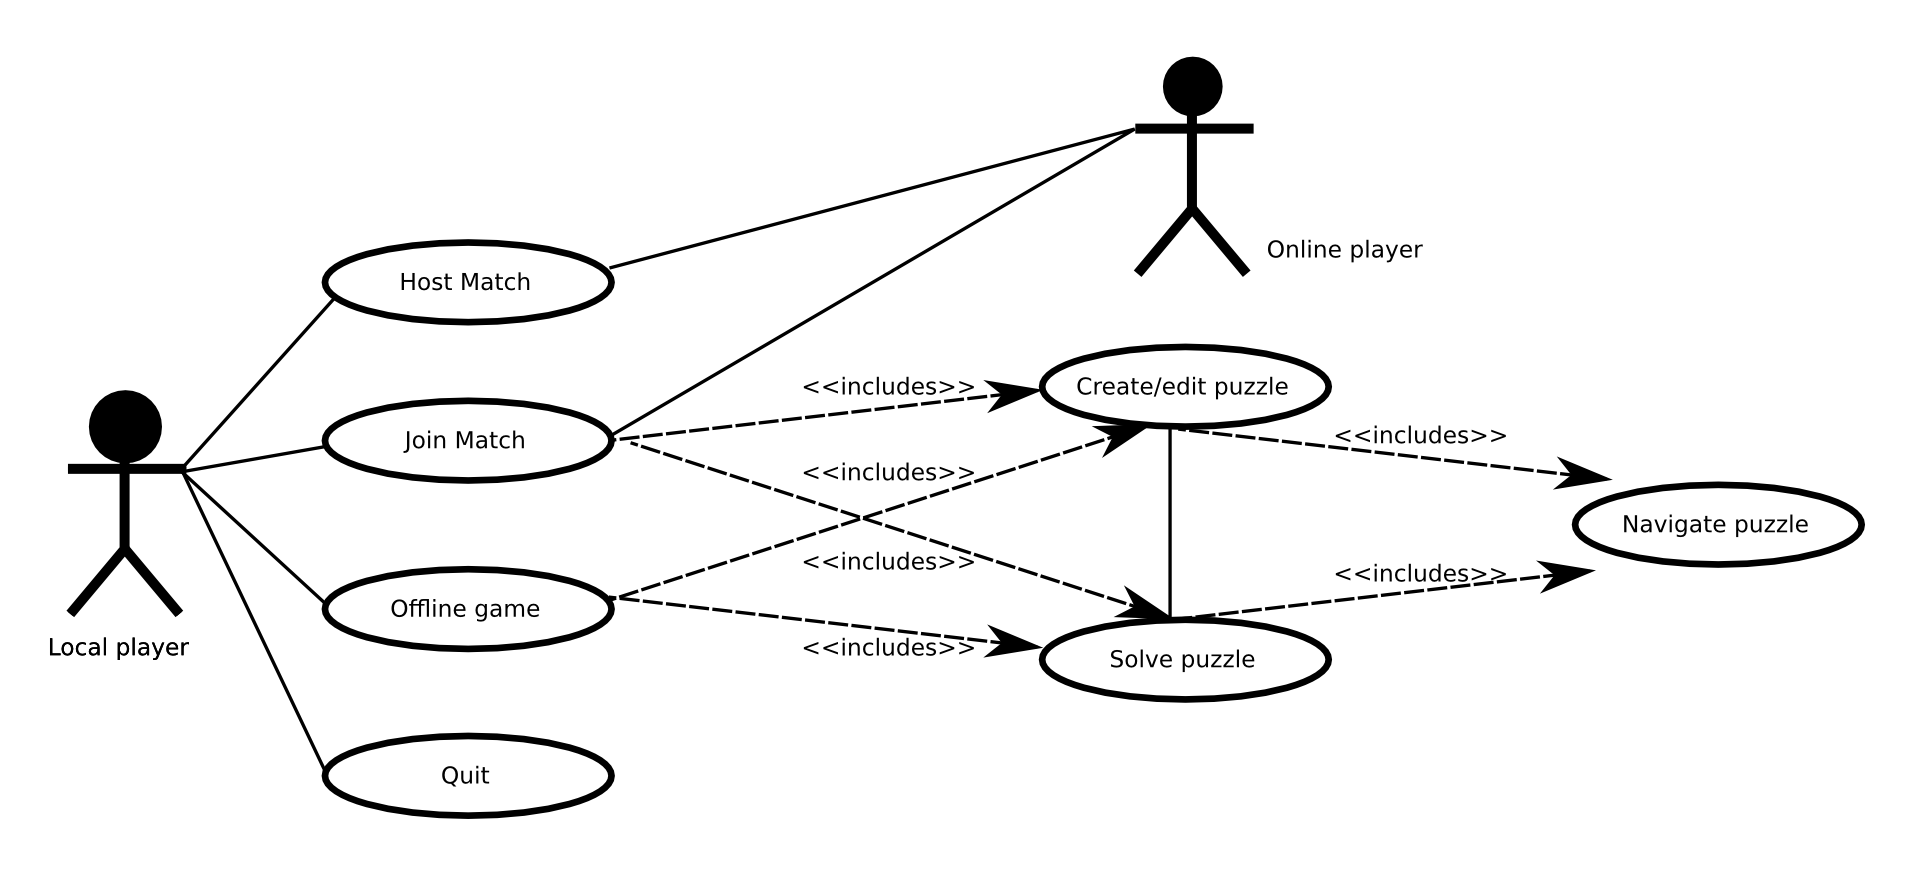
\includegraphics[width=6in]{use_cases.png}
        \caption{Use Case Diagram}
    \end{figure}

\subsection{Actor Descriptions}
    \begin{description}
        \item[Local player] is the local user and has full
            access to the mouse and keyboard or touchscreen interface.
        \item[Online player] is a non-local player. There is two-way
            communication between this type of player and the local player.
            There may be 0 or more online players.
        \item[The Host] has special powers, may disconnect other players and
            block players from selecting different puzzles. This player could
            be Local or Online.
    \end{description}

\subsection{Use-case Descriptions}
\begin{mdframed}
    \subsubsection{Host match}
    \begin{description}
        \item[Entry conditions] Internet connection.
        \item[Exit conditions] Will return to game menu. All players
            disconnected or all puzzles have been solved.
% NOPE on one solution
        \item[Participating Actors] Online player and local player.
        \item[Flow of events]:
            \begin{enumerate}
                \item The user presses the appropriate menu button.
                \item User creates a game, selects number of players and game
                    type

% NOPE could not complete. must share IP
                \item User shares (friendly looking) match ID with other
                    players. These players may connect to the match
                \item Puzzle Selector appears.
                \item The user may configure the game with this screen.
                    This
                    entails choosing a puzzle and a game mode (edit or solve).
                    Other players can be prevented from making such
                    modifications.
                \item This Puzzle Selector will create a Puzzle Scene
                \item The scene will change from the main menu to the Puzzle
                    Scene.
                \item Additional view-ports will be added to the game screen.
                These show the progress of online players by mirroring their
                puzzle behind and to the side of the local player's puzzle.

            \end{enumerate}
    \end{description}
\end{mdframed}

\begin{mdframed}
    \subsubsection{Join match}
    \begin{description}
        \item[Entry conditions] Internet connection. The menu must be present.
        \item[Exit conditions] Will return to game menu. All players
            disconnected or all puzzled have been solved.
        \item[Participating Actors] Online player and local player.
        \item[Flow of events]:
            \begin{enumerate}
                \item The user presses the appropriate menu button.
% NOPE could not complete. must receive map from host and not through puzzle selector
                \item This host will send a Puzzle Scene
                \item The scene will change from the main menu to the Puzzle
                    Scene.
                \item Additional view-ports will be added to the game screen.
                These show the progress of online players in the same way as
                the Host use case.
            \end{enumerate}
    \end{description}
\end{mdframed}


\begin{mdframed}
    \subsubsection{Offline game}
    \begin{description}
        \item[Entry conditions] Menu must be present.
        \item[Exit conditions] Will return to game menu. Puzzle has been
            solved or user wishes to return to the menu.
        \item[Participating Actors] Local player.
        \item[Flow of events]:
            \begin{enumerate}
                \item User selects the appropriate menu button.
                \item Puzzle Selector appears.
                \item The user may configure the game with this screen. This
                    entails choosing a puzzle and a game mode (edit or solve).
                \item This Puzzle Selector will create a Puzzle Scene
                \item The scene will change from the main menu to the Puzzle
                    Scene.
            \end{enumerate}
    \end{description}
\end{mdframed}


\begin{mdframed}
    This use case includes the Host Match, Join Match and Offline Game
    use cases.
    \subsubsection{Edit puzzle}
    \begin{description}
        \item[Entry conditions] A Puzzle Scene must be loaded and edit mode
            must be activated.
        \item[Exit conditions] Will return to game menu. The puzzle may be
            saved to the disk.
        \item[Participating Actors] Online player or local player.
        \item[Flow of events]:
            \begin{enumerate}
                \item The user navigates the puzzle
                \item If a position on the grid is selected, the Block Modifier
                    is presented. This position may be empty or it may
                    contain a block.
                \item The user may change properties of the block using this
                    screen.
                \item Blocks may be added or removed using this same screen.
            \end{enumerate}
            Puzzle preview:
            \begin{enumerate}
                \item User may press the preview button
                \item The user will try the puzzle in Solve Puzzle mode until
                    that mode's exit conditions are met.
                    A special banner will graphically indicate preview mode.
                \item The solving scene will have a special button for
                    returning to the editing scene
            \end{enumerate}
    \end{description}
\end{mdframed}


\begin{mdframed}
    This use case includes the Host Match, Join Match and Offline Game
    use cases.
    \subsubsection{Solve puzzle}
    \begin{description}
        \item[Entry conditions] A Puzzle Scene must be loaded and solve mode
            must be activated.
        \item[Exit conditions] Will return to game menu or puzzle editor.
            If the game is over, an overview of results will be shown and the
            steps taken to solve the puzzle may be saved to the disk.
        \item[Participating Actors] Online player or local player.
        \item[Flow of events]:
            \begin{enumerate}
                \item The user navigates the puzzle
                \item If a block is selected, the block runs any associated
                    Block Action.
                \item These Block Actions may modify the block's properties or
                    request the addition or removal of blocks, including the
                    selected block, from the Grid Manager.
                \item This sequence is repeated until the winning block is
                    found, the user quits, or a losing condition is met.
                \item User's actions may be mirrored on an online player's
                    screen, likewise, separate Puzzle Scenes  may be updated
                    with any moves made by other players.
            \end{enumerate}
    \end{description}
\end{mdframed}


\begin{mdframed}
    \subsubsection{Navigate puzzle}
    This use case includes the Solve puzzle and Edit puzzle use cases.
    \begin{description}
        \item[Entry conditions] Puzzle scene loaded and permission to move.
            Input devices must be functional.
        \item[Exit conditions] The game must offer continuous feedback.
            If the entry conditions are met, any further input must be
            acted on as soon as possible.
        \item[Participating Actors] Online player and local player.
        \item[Flow of events]:
        	\\
            Camera motion:
            \begin{enumerate}
                \item User drags with a mouse or touchscreen
                \item The camera changes position
            \end{enumerate}

            Block selection:
            \begin{enumerate}
                \item User clicks with mouse or taps on touchscreen
                \item The 3D coordinates are translated into a position on
                    a game ``board.''
                \item The Grid Manager is notified of input and the grid
                    position.
                \item If a block is present there, it is selected and activated.
                    Exact actions depend on the game mode.
                \item If a block is not present, the space is selected. This
                    is only useful in edit mode.
                \item The user may end the game at any point through the pause
                    menu.
            \end{enumerate}

    \end{description}
\end{mdframed}


\begin{mdframed}
    \subsubsection{Quit}
    \begin{description}
        \item[Entry conditions] Game must be running. This action is
            asynchronous and may activate at any point.
        \item[Exit conditions] Game, be gone!
        \item[Participating Actors] Local player.
        \item[Flow of events]:
            \begin{enumerate}
                \item User presses the quit button on a menu
                \item or User presses appropriate sequence of keys, such as
                    the escape key or the alt and F4 combo.
                \item Some data may be saved, such as the puzzle being currently
                edited.
                \item The program shuts down gracefully.
            \end{enumerate}
    \end{description}
\end{mdframed}



\section{Architectural Design}
% HR
% Briefly overview your architectural design. Discuss alternatives examined. Indicate why the
% architecture discussed in section 3.1 & 3.2 was chosen and why the alternatives were eliminated.

We chose the file-system to save persistent data, a single game program with
both client and host modes as a networking model, and the Godot Engine for most tasks.

The file-system is the easiest and most portable method to save data. It is
suited to the game's few storage requirements. We only need to save scores,
custom levels and settings.

The user decides at the game menu whether to host a game or join a game, this
dynamic approach is convenient for the user; a dedicated server
would be too difficult for this casual game. A peer-to-peer solution would
also be easy for the user, but Godot has better support for the Server/Client
model.

We also considered using Unity, Ogre, Irrlicht, and Three.js for our
game. All of these game engines can generate portable executables, but Godot
was chosen thanks to its multi-platform development environment, unlike Unity;
a complete set of libraries, unlike Irlicht and Ogre; speed of execution,
unlike Three.js. Only Three.js and Godot support mobile platforms.
Three.js and Unity were the closest contenders.



\subsection{Subsystem Architecture}
% SM
\begin{figure}[H]
    \centering
    
\includegraphics[width=0.8\linewidth]{subsys_arch.png}
    \caption{Layered Subsystem Architecture UML Diagram.}
\end{figure}
The two primary subsystems of Anttris are the puzzle system and the online system.

The puzzle-solving system is composed generically over a puzzle viewer and attached event
handling that allows interaction with the puzzle. Both offline games and online ones use
the puzzle viewer, as does the unique puzzle-editing mode. The puzzle viewer is used by
all three unique modes, and works with our 3D model interaction system to provide
interactivity. This system is built on the Godot 3d Engine, which uses OpenGL.

The online system breaks down immediately into host mode or remote client mode. The host
mode interfaces with the application-generic session-host system, which works in conjunction
with the session lobby to facilitate remote clients to connect and play against the host.
Remote clients also work closely with the session lobby to find hosts to play against. Both
the session lobby and the session-host system work with the Godot Online Subsystem to provide
connectivity. The Godot Online Subsystem is built over TCP-UDP/IP.

\subsection{Deployment Model}
% HR
We have a simple deployment scheme: install the same game on compatible systems
and allow the user to dynamically choose the session type. There will be
one host machine and zero or more client machines. A game in offline mode is
treated as a host machine.
    \begin{figure}[H]
        \centering
        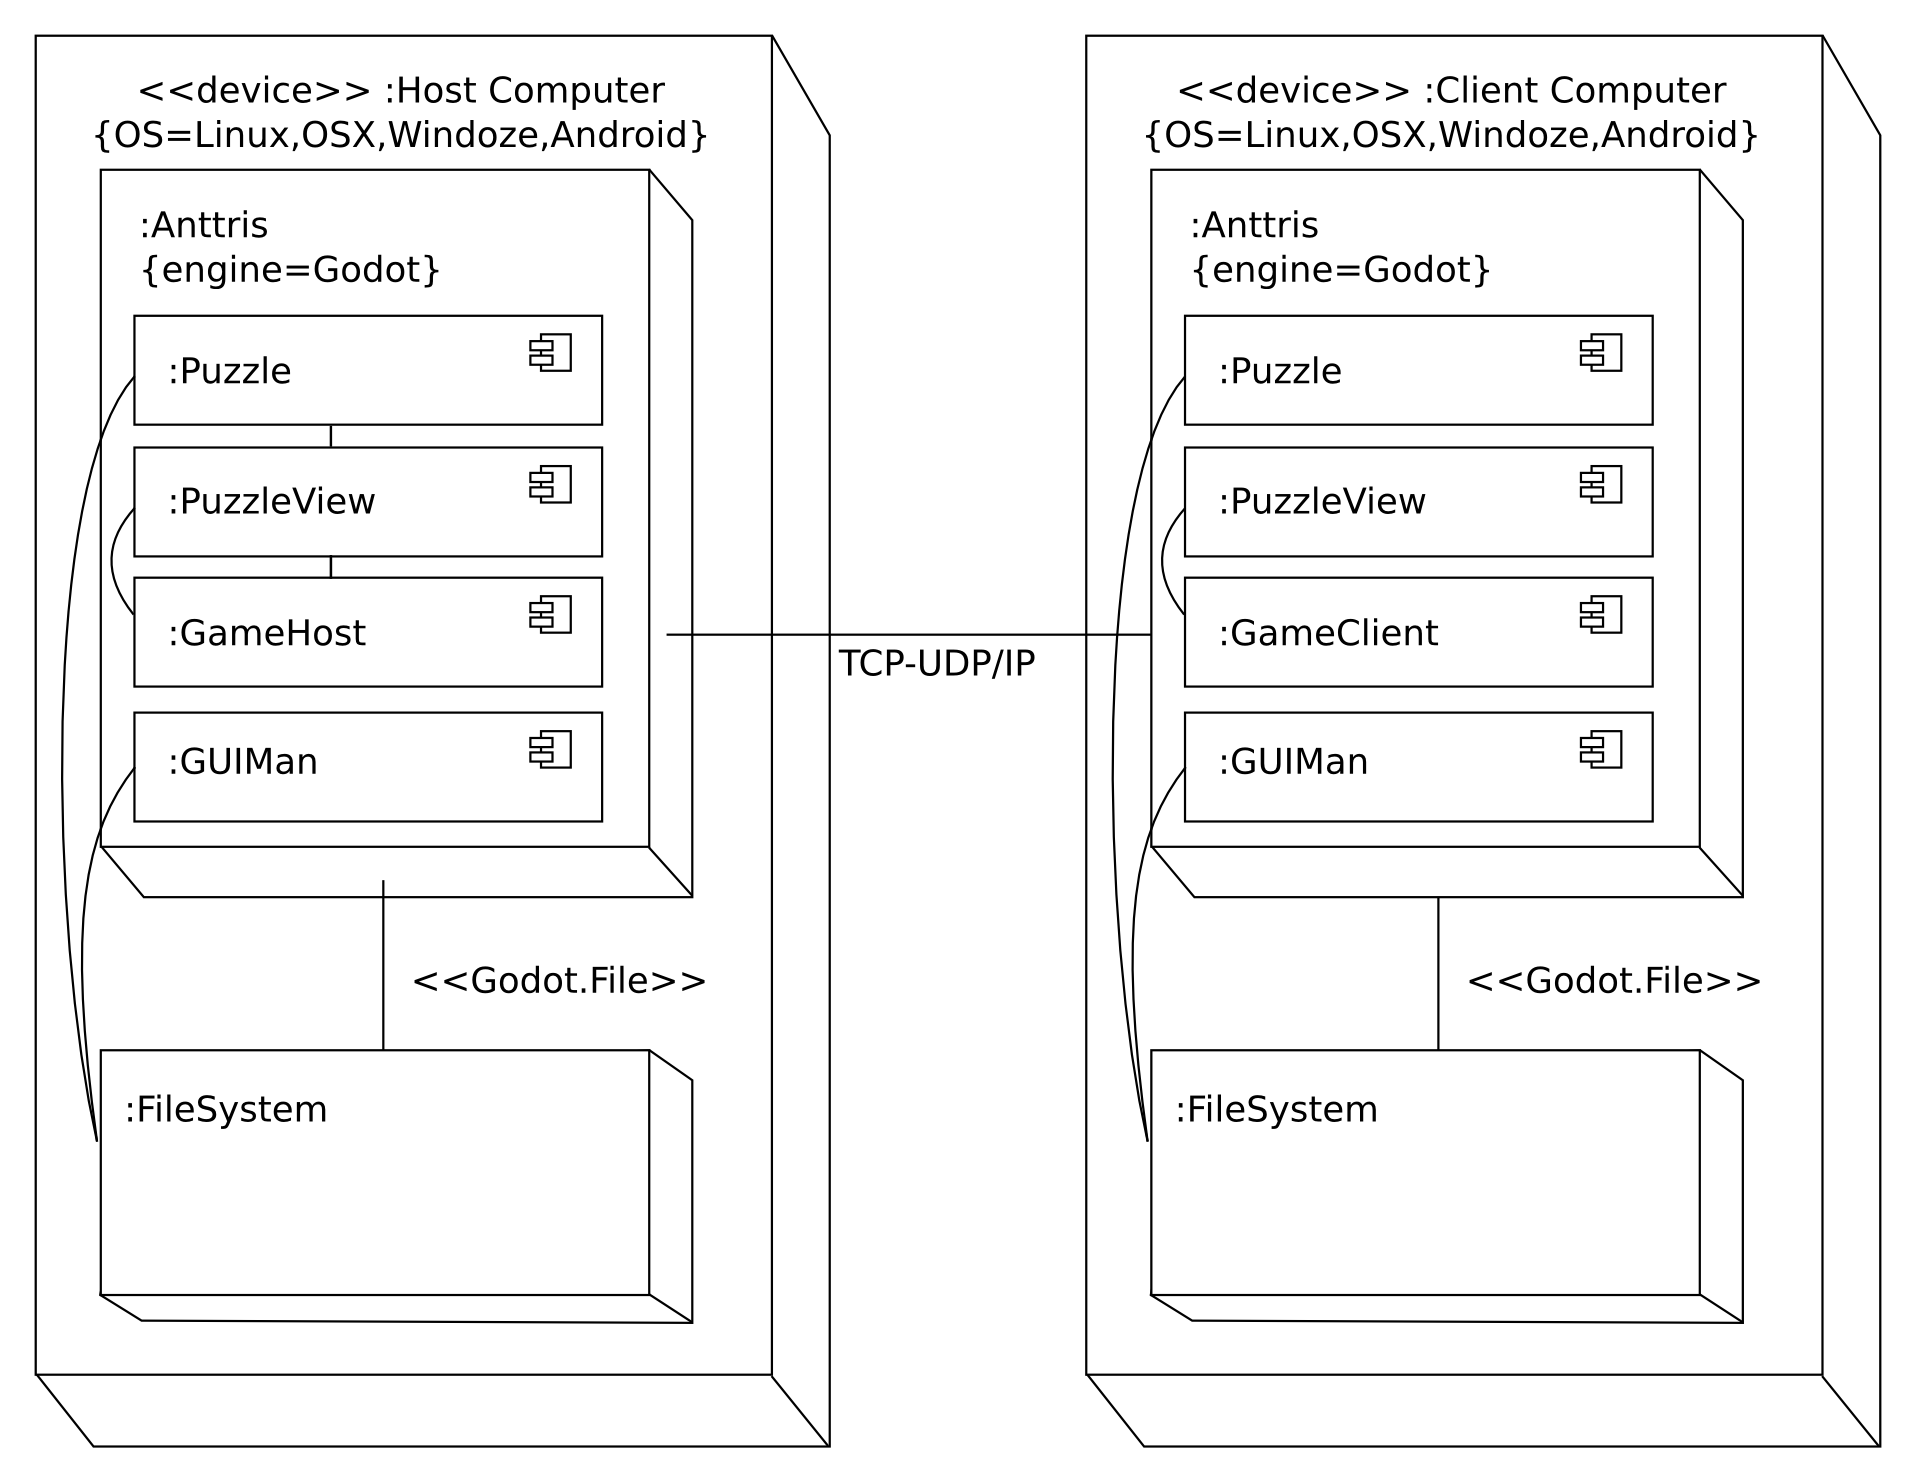
\includegraphics[width=6in]{deployment_diagram.png}
        \caption{Deployment diagram. Installation is the same for both host and
        client. The type of session is chosen dynamically by the user}
    \end{figure}

\section{Use Case Realization Design}
% HR, I did Use Cases last time, I can work on all of this
Every significant use case will be realized here using both class diagrams and
sequence diagrams. Notice the OfflineGame use case can be modeled by a Host
with no clients, no further elaboration is needed for that. The Quit use case
is trivial.

\subsection{Sequence Diagrams}
\foreach \n/\desc in {%
{{sequence_edit.png%
}/{Sequence Diagram for editing a puzzle}},
{{sequence_join_match.png%
}/{Sequence Diagram for joining a match    }},
{{sequence_solve.png%
}/{Sequence Diagram for solving a puzzle  }},
{{sequence_host_match.png%
}/{Sequence Diagram for hosting a match  }},
{{sequence_navigate_puzzle.png%
}/{Sequence Diagram  for navigating the puzzle}}}
{%
    \begin{figure}[H]
        \centering
        \includegraphics[width=0.7\textwidth]{\n}\par
        \caption{\desc}
    \end{figure}
}

\subsection{Class Diagrams}

\foreach \n/\desc in {%
{{class_edit.png%
}/{UML Class diagram for the puzzle editing Use Case. Notice TestGame is used
to start a new GameEngine to test the current puzzle.}},
{{class_join.png%
}/{UML Class diagram for a client joining a game.}},
{{class_solve.png%
}/{UML Class diagram for solving the game. }},
{{class_host.png%
}/{UML Class diagram for hosting a game.}},
{{class_navigate.png%
}/{UML Class diagram for navigating the puzzle.}}}
{%
    \begin{figure}[H]
        \centering
        \includegraphics[width=0.7\textwidth]{\n}\par
        \caption{\desc}
    \end{figure}
}

\section{Subsystem Design} % CA
Anttris is broken down into the following four subsytems: GUI, Networking, File Manager and Game.
\subsection{Anttris GUI} % CA
    \begin{figure}[H]
        \centering
        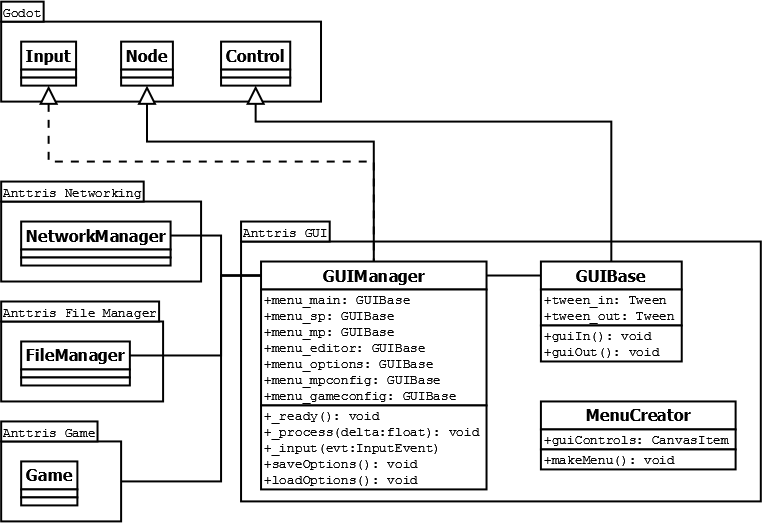
\includegraphics[width=6in]{Anttris_GUIClass.png}
        \caption{Class diagram for the GUI subsystem.}
    \end{figure}
    \begin{figure}[H]
        \centering
        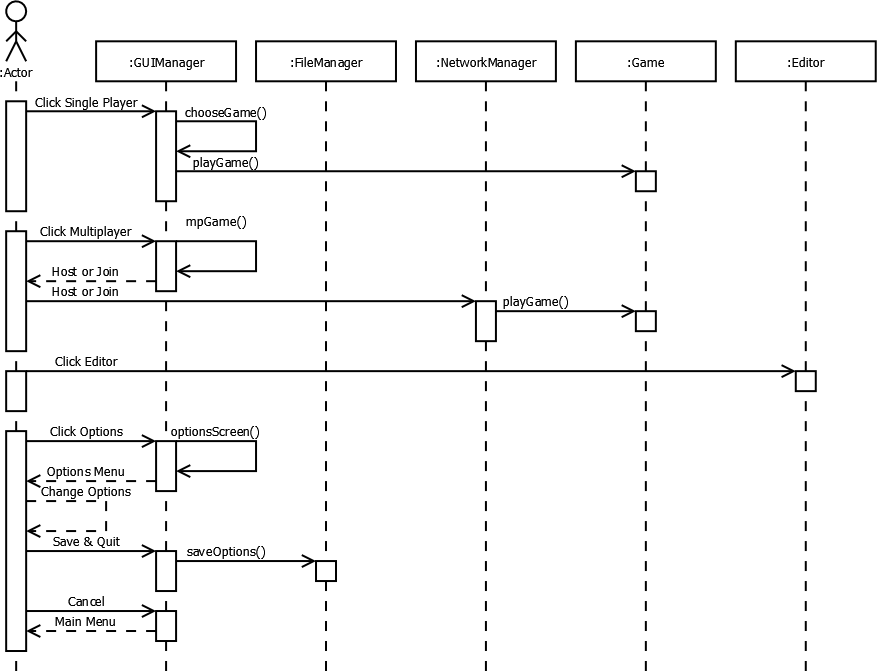
\includegraphics[width=6in]{Anttris_GUISequence.png}
        \caption{Sequence diagram for the GUI subsystem.}
    \end{figure}

This subsystem manages all of the graphical user interfaces that make up the menus. Menus all inherit GUIBase to provide smooth and consistent fade in and slide out animations. The MenuCreator just takes all of the buttons in a menu and orders them nicely for consistency. The menus themselves will be object instances of GUIBase.

\subsection{Anttris Game Engine} % CA
    \begin{figure}[H]
        \centering
        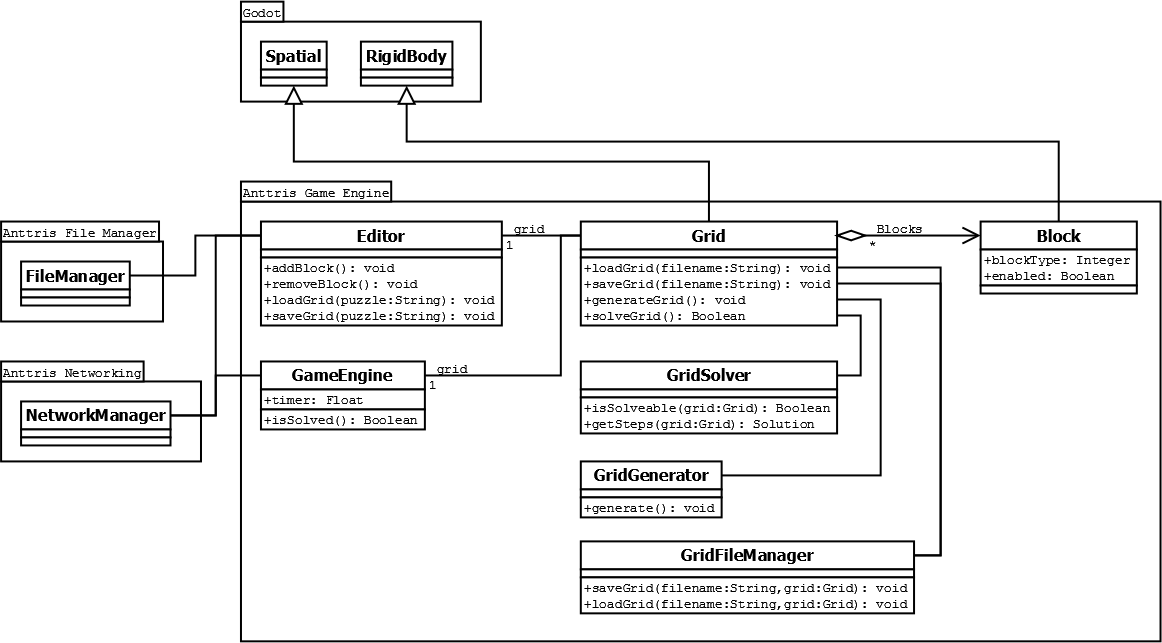
\includegraphics[width=6in]{Anttris_GameClass.png}
        \caption{Class diagram for the game subsystem.}
    \end{figure}
	\begin{figure}[H]
        \centering
        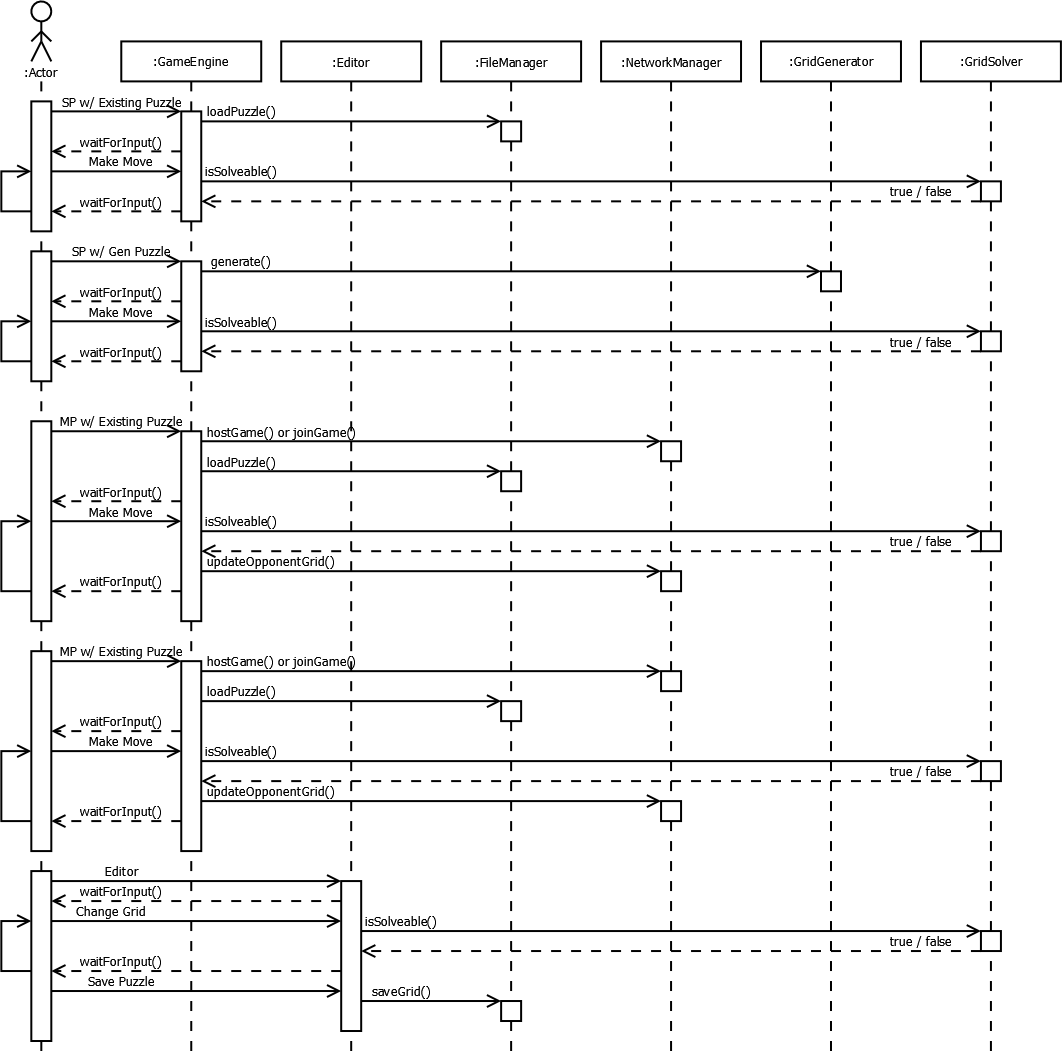
\includegraphics[width=6in]{Anttris_GameSequence.png}
        \caption{Sequence diagram for the game engine subsystem.}
    \end{figure}

This subsystem manages all of the game and editor states. The game and editor are similar with minor differences in input. This subsystem handles both single player and competitive modes.

\subsection{Anttris Network Manager} % CA
    \begin{figure}[H]
        \centering
        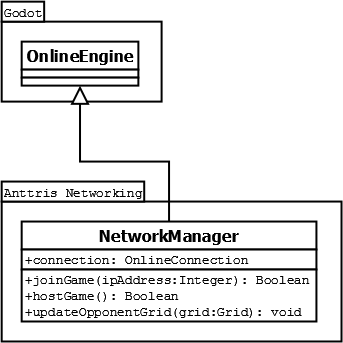
\includegraphics[width=2.7in]{Anttris_NetworkingClass.png}
        \caption{Class diagram for the networking subsystem.}
    \end{figure}

This subsystem will provide a central interface for networking. All games that are joined or hosted for competitive play will go through this subsystem. It updates the connection periodically and updates the opponents grid on the screen when they make new moves. This subsystem has no sequence diagram as it is self contained and is only used by outside subsystems. See the sequence diagrams for the GUI and game subsystems.

\subsection{Anttris File Manager} % CA
    \begin{figure}[H]
        \centering
        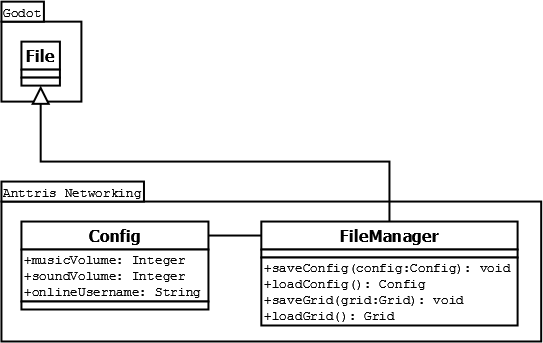
\includegraphics[width=4.27in]{Anttris_FileClass.png}
        \caption{Class diagram for the file management system.}
    \end{figure}

This subsystem provides a central interface for file management. Options are be loaded and saved from here as well as any puzzles created in the editor.
\section{Human Interfaces} % CA / SM
Screenshots included below are final in-game designs.
	\begin{figure}[H]
        \centering
        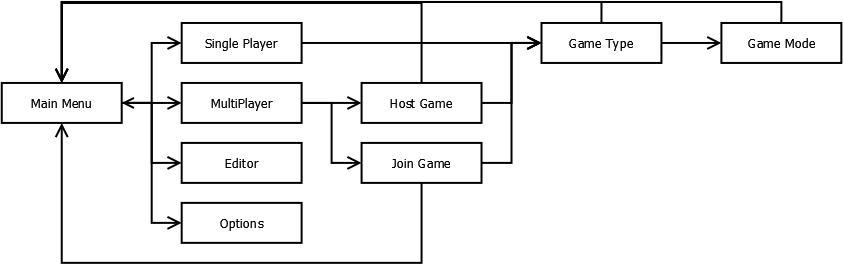
\includegraphics[width=4.5in]{Anttris_MenuFlow.png}
        \caption{Overall flow of the GUI.}
    \end{figure}
    \begin{figure}[H]
        \centering
        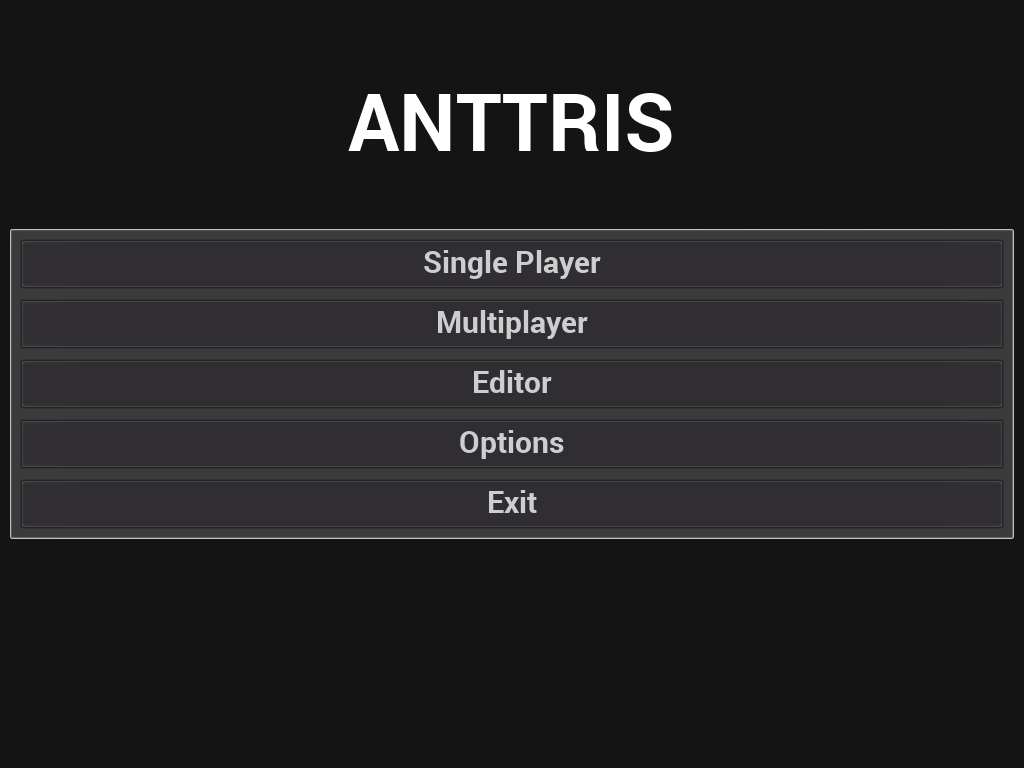
\includegraphics[width=4.5in]{Anttris_MainMenu.png}
        \caption{Main menu design.}
    \end{figure}
    \begin{figure}[H]
        \centering
        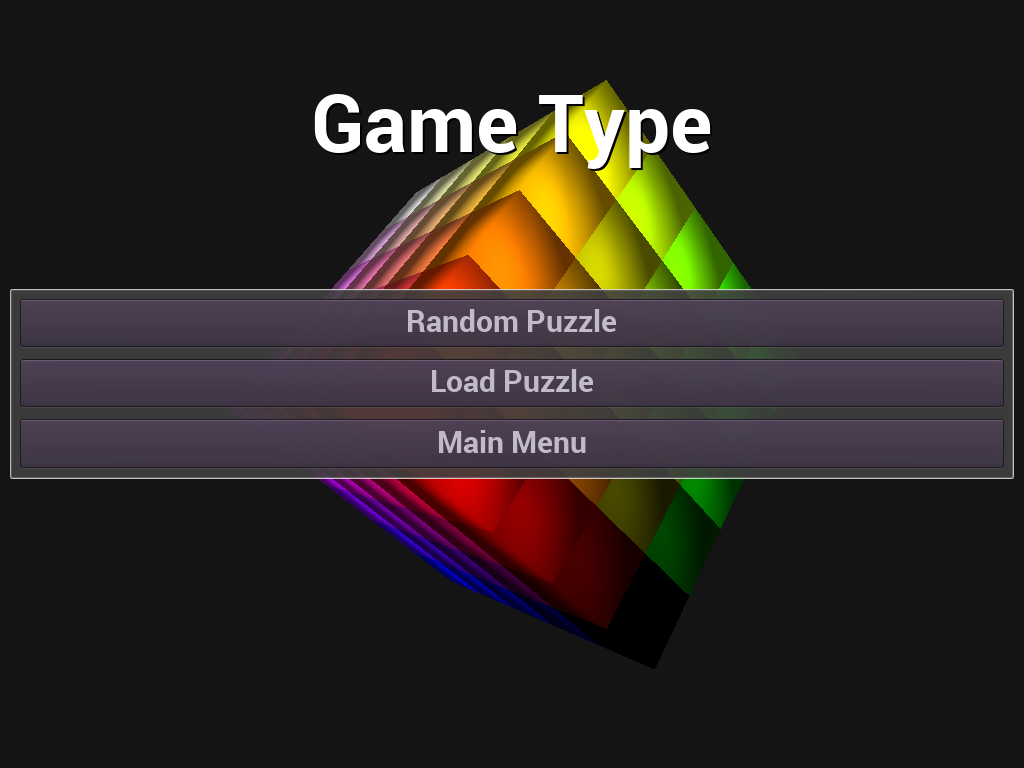
\includegraphics[width=4.5in]{Anttris_GTMenu.png}
        \caption{Game type menu design.}
    \end{figure}
    \begin{figure}[H]
        \centering
        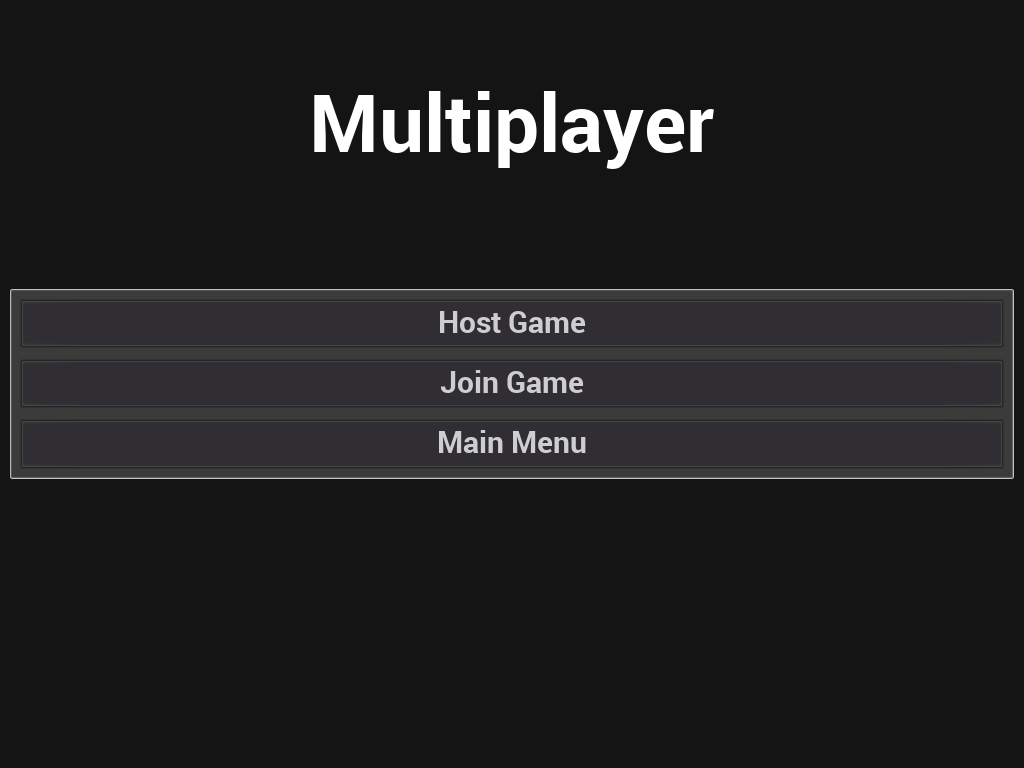
\includegraphics[width=4.5in]{Anttris_MPMenu.png}
        \caption{Multiplayer menu design.}
    \end{figure}
    \begin{figure}[H]
        \centering
        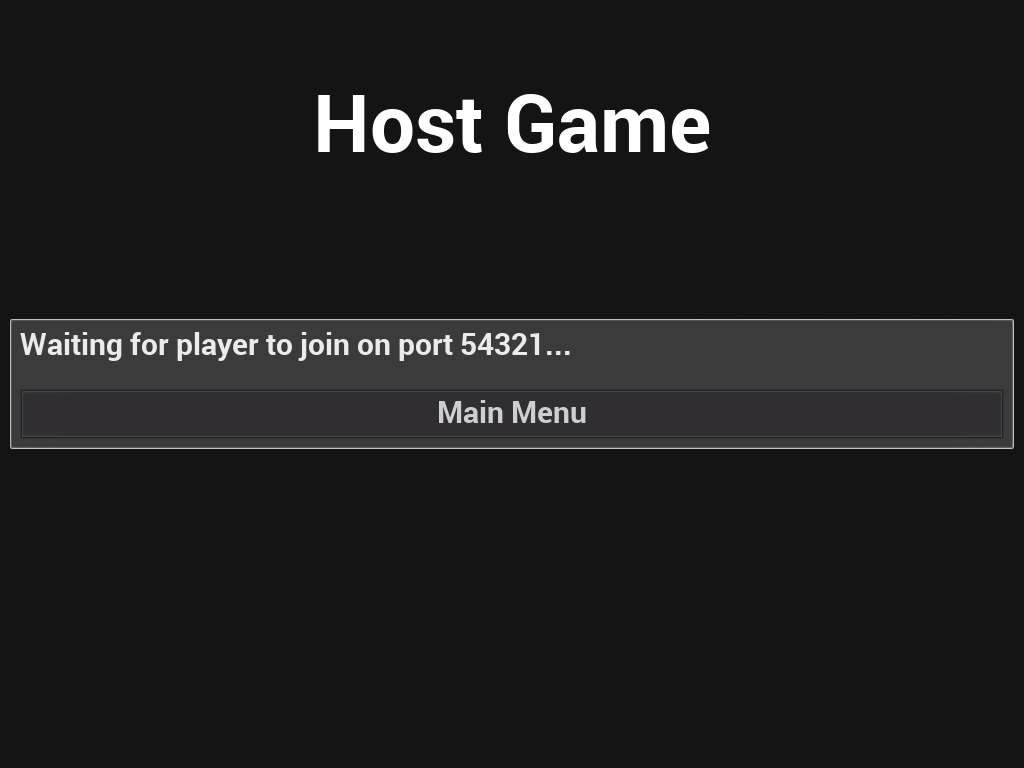
\includegraphics[width=4.5in]{Anttris_HGMenu.png}
        \caption{Host game menu design.}
    \end{figure}
    \begin{figure}[H]
        \centering
        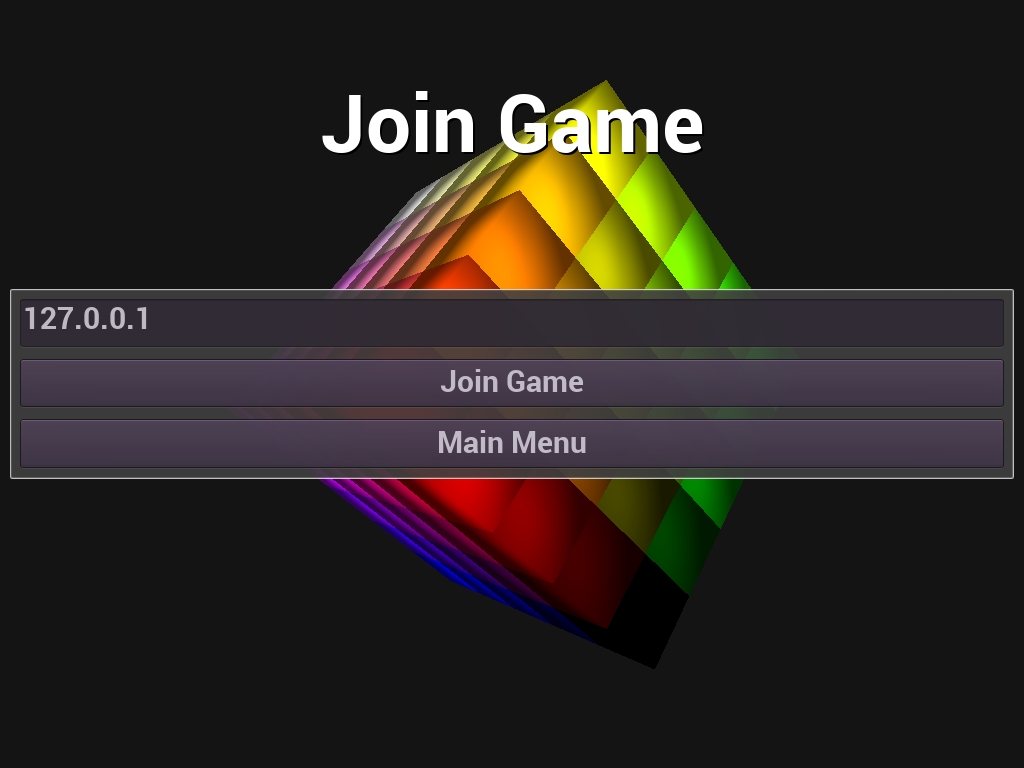
\includegraphics[width=4.5in]{Anttris_JGMenu.png}
        \caption{Join game menu design.}
    \end{figure}
    \begin{figure}[H]
        \centering
        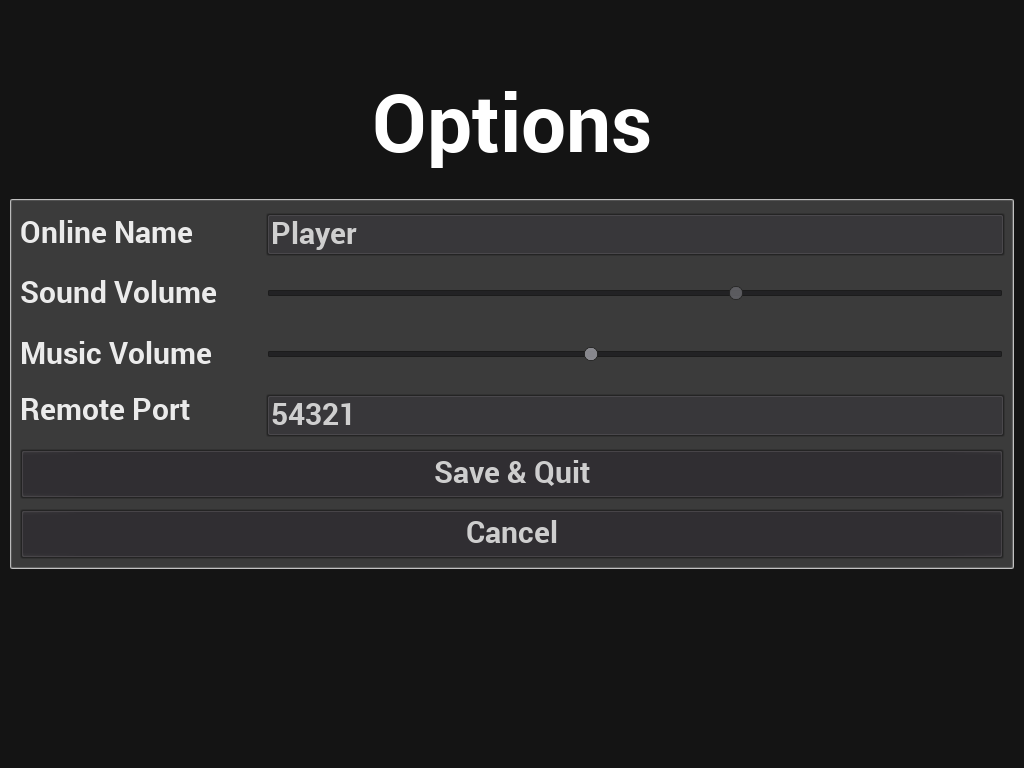
\includegraphics[width=4.5in]{Anttris_OptionsMenu.png}
        \caption{Options menu design.}
    \end{figure}
\section{System/Data Dependencies \& Requirements}
% edited by ST
In order for a user to play Anttris, the user will need a personal computer with a modern graphics card, a mouse, and keyboard. The computer will need to be a standard x86 machine---running Windows, Mac, or GNU/Linux---that is up to date in order to play the game.
The graphics card needs to be reasonably modern since it must provide a minimum of 30 frames per second. Most recent desktop and mobile cards should be able to achieve this. The mouse and keyboard are the primary input devices.

A user may also choose to play Anttris on a mobile device, in which the device is a smart phone, running either the Android or iOS operating system. The phone's operating system will need to be up to date in order to play the game effectively. The touch screen of the device will be used to input commands into the game.

In order for the user to play multiplayer matches, the user will need an internet connection and IP address for their personal computer or mobile phone in order to connect to the other user. The user can still play the game in single-player mode which does not require internet access, however game play will be limited.

Anttris will need filesystem access in order to create, write, and modify save data and scores for each puzzle. Additionally, the Puzzle Editor will need to be able to read and write data for user-generated puzzles.
% ST, BC
\section{Testing Plan \& Results}
% Must revise this after actually running tests

In order to test that the game is working properly we will be using Black Box and White Box testing methods. Using these methods we can test the game from the outside-in by making sure that the functionality of the interface preforms the correct actions then working our way to the coding level. This approach will prevent more errors and bugs in the early stages of testing, since we will not be working with the code directly at the start. Any errors and bugs we encounter will be documented and recorded for future reference.

Our testing plan is as follows:
\begin{enumerate}
\item Black Box Testing
\item White Box Testing
\item User Testing
\end{enumerate}

For the first part of the testing plan, we will be testing the game on multiple physical computers to make sure the interface of the game preforms correctly. Testing the game on multiple machines will allow for a diverse testing experience, and will confirm whether or not our game can work on multiple systems. Once we know the game can run on each of the tested machines, we will begin testing the interface of the game.
The interface of the game is what the user will be interacting with, so we want to make sure that the interactions of each function work correctly and display the correct information to the user. To test the interface of the game we will:

\begin{enumerate}
\item Test the menu options
\item Test single-player Game Mode (Single-player, New Game, Continue Game)
\item Test Puzzle Editor/Creator: (Create, Edit, Delete)
\item Solve basic test puzzles (Test Puzzle 1, 2, 3\dots)
\item Multiplayer Game Mode
\end{enumerate}

After testing the interface of the game and making sure each of the game options and modes work correctly, we will review errors and bugs we encountered during the Black Box testing. Upon completion we will need to begin White Box testing and testing that the correct values are being passed in the code.

\subsection{Testing Menu Options}
In order to test the menu options, we will click on each of the options and make sure that the selected menu option displays the next options or pages the user needs to see. For instance, if a user selects “single-player game”, we don't want the game pulling up the information for a multiplayer game.
We will be testing each of the options the user may choose from and if the user can reselect options by returning to the previous options. Since this is the first thing the user will see when playing our game, and is what decides what type of games the user will be playing, we can to make sure they work properly and don't cause the game to close unexpectedly.

\subsection{Test Single-Player Mode}
Once we know all the menu options work correctly, we will test the single-player Game Mode. In single-player, the user will be able to select whether they wish to start a new game or continue a game they left off on. The New Game option will allow the user to select the puzzle they wish to play and solve that puzzle from the beginning. In order to test this option, we will have a set number of puzzles generated and we will test each puzzle separately on each machine. We want to make sure that the puzzle generates the correct puzzle and generates the same way each time. After testing the new game function, we will test the continue function. This function allows the user to continue from a saved game file and will allow the user to continue solving the puzzle.

\subsection{Test Puzzle Editor/Creator}
After we have tested the New Game and Continue functions, we will be testing the puzzle editor functions which are accessed in the single-player Mode. The puzzle editor is where the user can create new puzzles, edit previously made puzzles, and delete puzzles they may not want anymore. In order to test creating new puzzles, we will be creating basic puzzles, seeing if we are allowed to place blocks on the grid correctly, and if the game will catch any errors when saving the puzzle. When creating basic puzzles we will be using the in game tools to create and remove blocks on the grid. We will need to test that we can place each type of block, and be able to remove each type of block when placed on the grid.
Testing the edit puzzle option is similar to the create new puzzle option, except when editing a puzzle we need to make sure that the puzzle the user wishes to edit appears correctly so the user can make the proper changes.

\subsection{Solving Puzzles}
After we have tested the Puzzle Editor, we will attempt to solve puzzles. Using per-constructed, basic puzzles, we will solve each of the puzzles and confirm that each of the blocks preforms the correct action when clicked, and test if the game records scores correctly and ends when the goal block is reached. Each of the tester puzzles, will consist of each type of block and possible interactions so we can make sure that the game flow is not ruined when blocks preform their actions. Solving Puzzles is the last step in testing the single-player mode and is the most important.

\subsection{Multiplayer Game Mode}
Multiplayer Game Mode will be the last thing we test since it involves the interactions between two computers. We will be testing the Create and Host Match options like we did the menu options and the different game modes similarly to the single-player and Multiplayer game modes. The most important thing we need to test for the multiplayer are the interactions between the two players. In order to test the interactions, we need to make sure that two players are able to connect to each other and preform actions in the interface and when solving puzzles with each other.

\subsection{White Box Testing}
The second part of the testing plan, we will be using the White Box testing method in which we will be dealing with the actual code of the game. We need to make sure that the code of the game is working correctly.
Changes to the code will be based on the errors and bugs we find during the black box testing. We will be treating the code as units and fixing only the function or object that needs fixing then reintegrating it back into the code. After reintegrating the newly fixed code, we will need to test the section of the game that we made changes to. For instance if we need to make changes to the way a tool works in the puzzle creator, we will make the change to the tool and test only the puzzle creator section of the game.
By making changes and fixing problems with the documented bugs and errors, and breaking the code into units, we will be able to efficiently make the necessary changes to the game. Once a group of changes have been made, we will test the game again using black box testing in order to make sure that the changes we made to the game did not affect any of the other section of the game. If any errors or bugs are found, they will be documented and recorded and any necessary changes will be made, and they will be tested again on the physical machine. After these changes have been implemented and test effectively, we will move on to the next stage of testing; user testing.

\subsection{User Testing}
The last part of our testing plan is user testing. User testing will allow for varying users to test the game and provide feedback about the game. This method of testing will help us gather information and discovery any bugs or errors that we could not find during the earlier parts of testing. For this part, we will ask a variety of users to test the game and fill out a survey generated by us. A few of the questions on the survey will ask about how the complexity, enjoyability, functionality, of the game and if the user came across any bugs or errors while playing the game. Using the survey, we can make any changes necessary to ensure the game is fully functional and working properly before we present our final product.
% ST, BC

\section{Project Status and Summary}
\subsection{Project Status} % SKYLER
% (What is and is not working. Was the plan maintained? Was the project modified from the original proposal? Etc.)
Anttris began with many features in mind. Through the course of the development of Anttris, these features remained our central focus. Elements like competitive multiplayer and the puzzle editor were required to give the game the substance needed to make it a great game instead of just some puzzle game.

All of the main features we planned for the game to have were successfully implemented. Features like single player and the editor have been created and thoroughly tested. Multiplayer games can be hosted and played with friends. Players can save and load blocks. Every feature planned out in the beggining was successfully added and tested in the game.

In addition, Anttris has an official game website! The website features explainations of the game rules, convenient download links, and screenshots of the game. The website was developed by us, and can be viewed by pointing a browser at
$$
http://gamewizards/github.io
$$

Finally, Anttris was built using git and GitHub. This means that the whole Anttris development process and final code is available for download at
$$http://github.com/gamewizards/anttris/$$
\subsection{Difficulties Encountered} % CHRIS
%(Include how they were managed or mitigated)
Throughout the project's development, we experienced a few minor difficulties. Although we experienced difficulties, out design principles allowed for us to dynamically change our design and quickly integrate new ideas to fix old ones.

The biggest issue we ran into involved the game's original rules. While the rules were a neat idea, determining the solvability of a puzzle proved to be an NP-hard problem. After realizing the complexity of solving puzzles, we simplified the rules in a way that was interesting, fun and could be solved.

Another difficulty we had involved the Godot Game Engine used to implement Anttris. The software is still currently in Beta and as such, there are still minor issues throughout the application. Most of these issues were solved through digging into Godot's source code or by finding workarounds.
\subsection{Journal of Project Activities} % SEAN
%(This is your group journal)
% add Github commit logs?
Team organization was important, so we organized weekly in-person meetings at various locations on campus. Most commonly we used Cramer 213, but also met in the library a few times. For all other times, we had all team communications centralized to Slack, so that everyone could talk to the team in an organized manner at any time of the day, as well as get centralized notifications from Github and Travis CI.

We used a modified Scrum methodology to organize the project. Agile development is great, but the normal schedules used by Agile teams are not necessarily optimal for students, so we settled on mainly using sprints as general guidelines for milestones. We also did not use daily in person standups, preferring instead to utilize Slack to talk constantly about what we were doing.

\subsubsection{Project Statistics}
Below are some figures taken from both Slack (communication statistics) and Github (coding statistics.) Please note that Github unfortunately only reports statistics for the default branch (in our case, master.) Thus, this data may not accurately reflect work put into branches. This is particularly true of Figure \ref{code:freq}, as it reflects a lot of the code that was merged into master towards the end of the project cycle. Additionally, Figure \ref{code:graph} is the state of the network graph on April 28 at about 10 PM. It will probably change a bit as more work is done, but it reflects how our branches have been fitting together.

\begin{figure}[H]
        \centering
        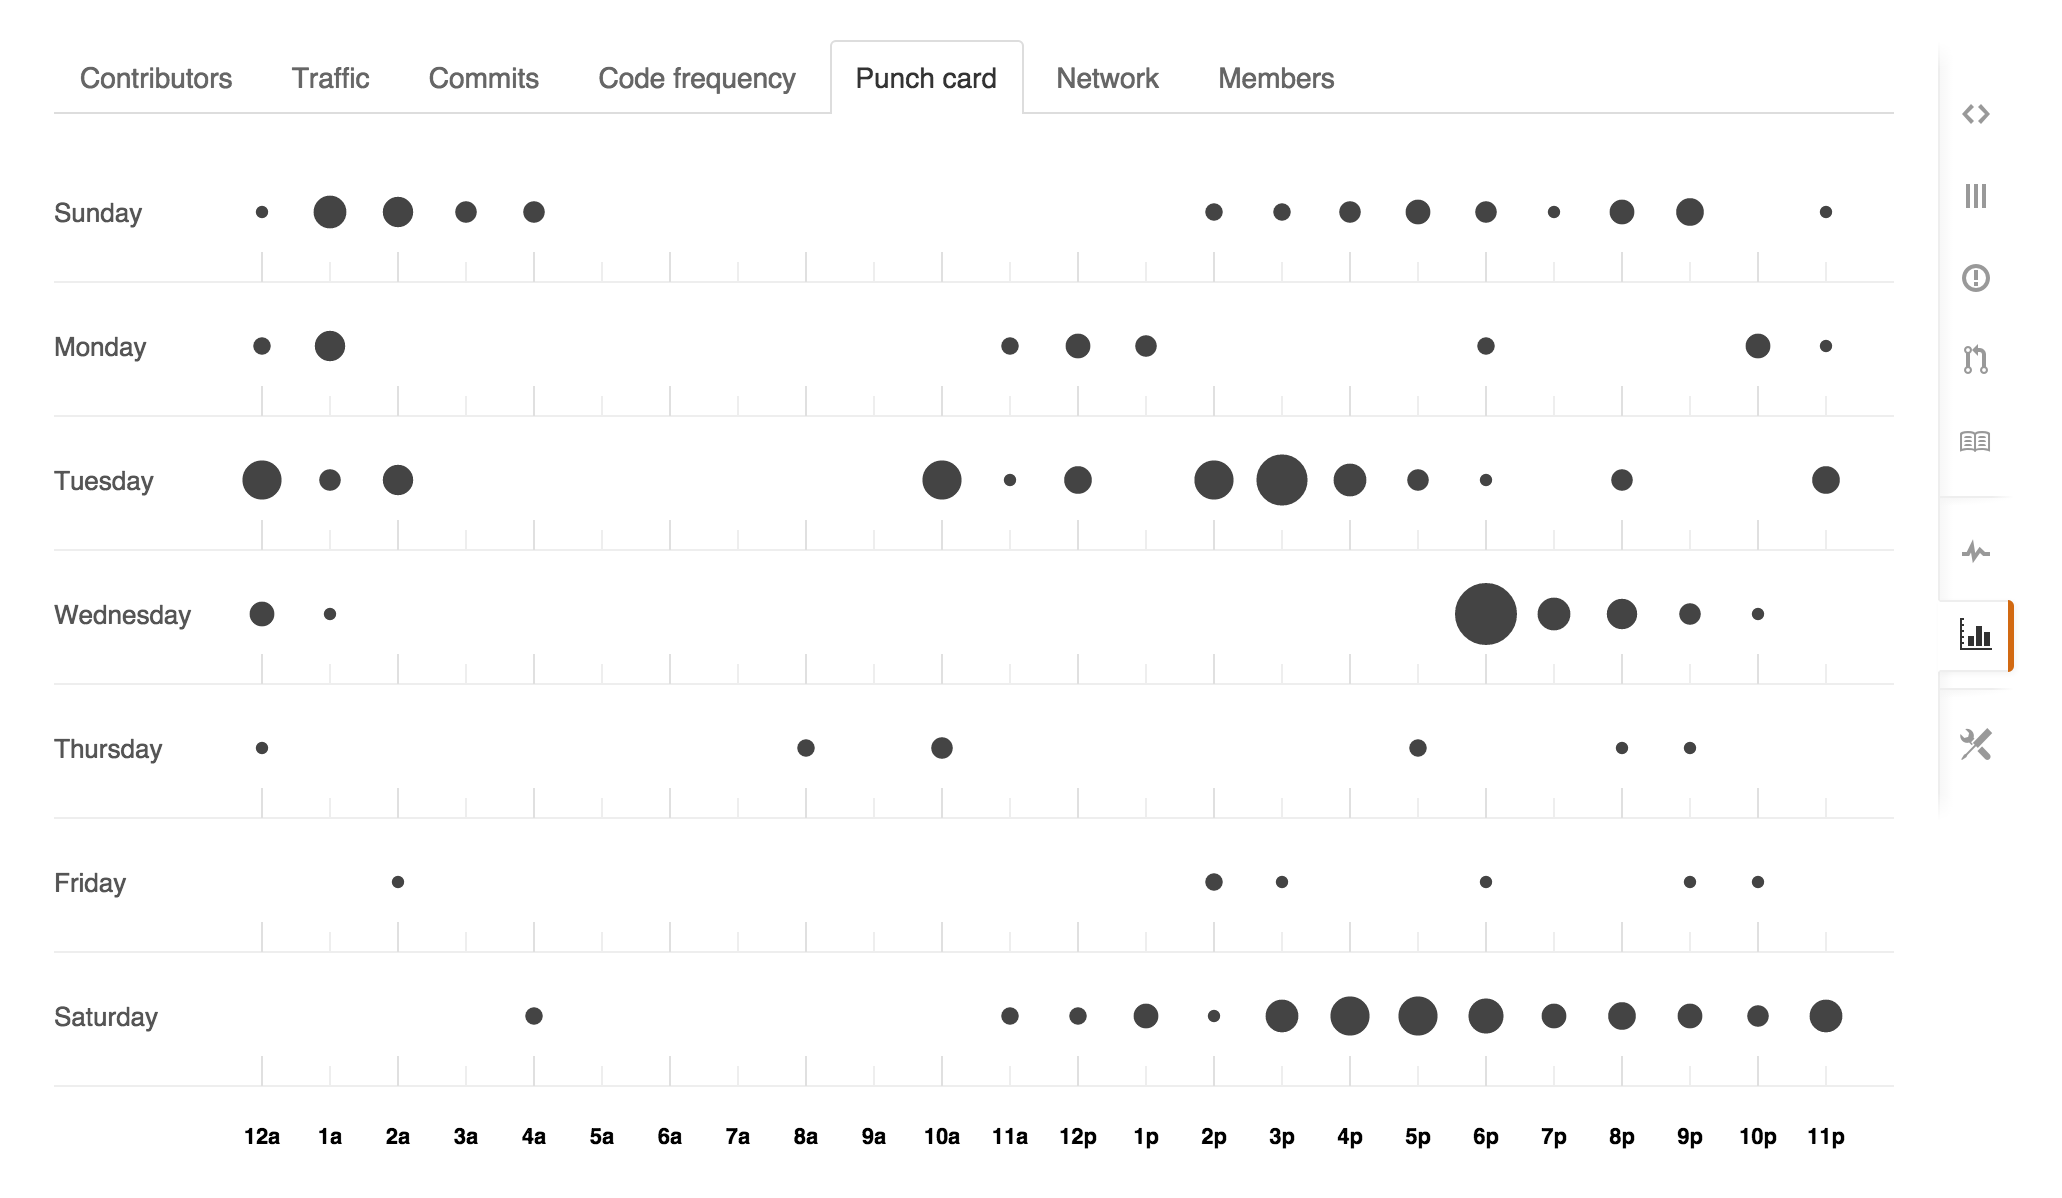
\includegraphics[width=4.5in]{punchcard.png}
        \caption{Github Punchcard}
\end{figure}

\begin{figure}[H]
        \centering
        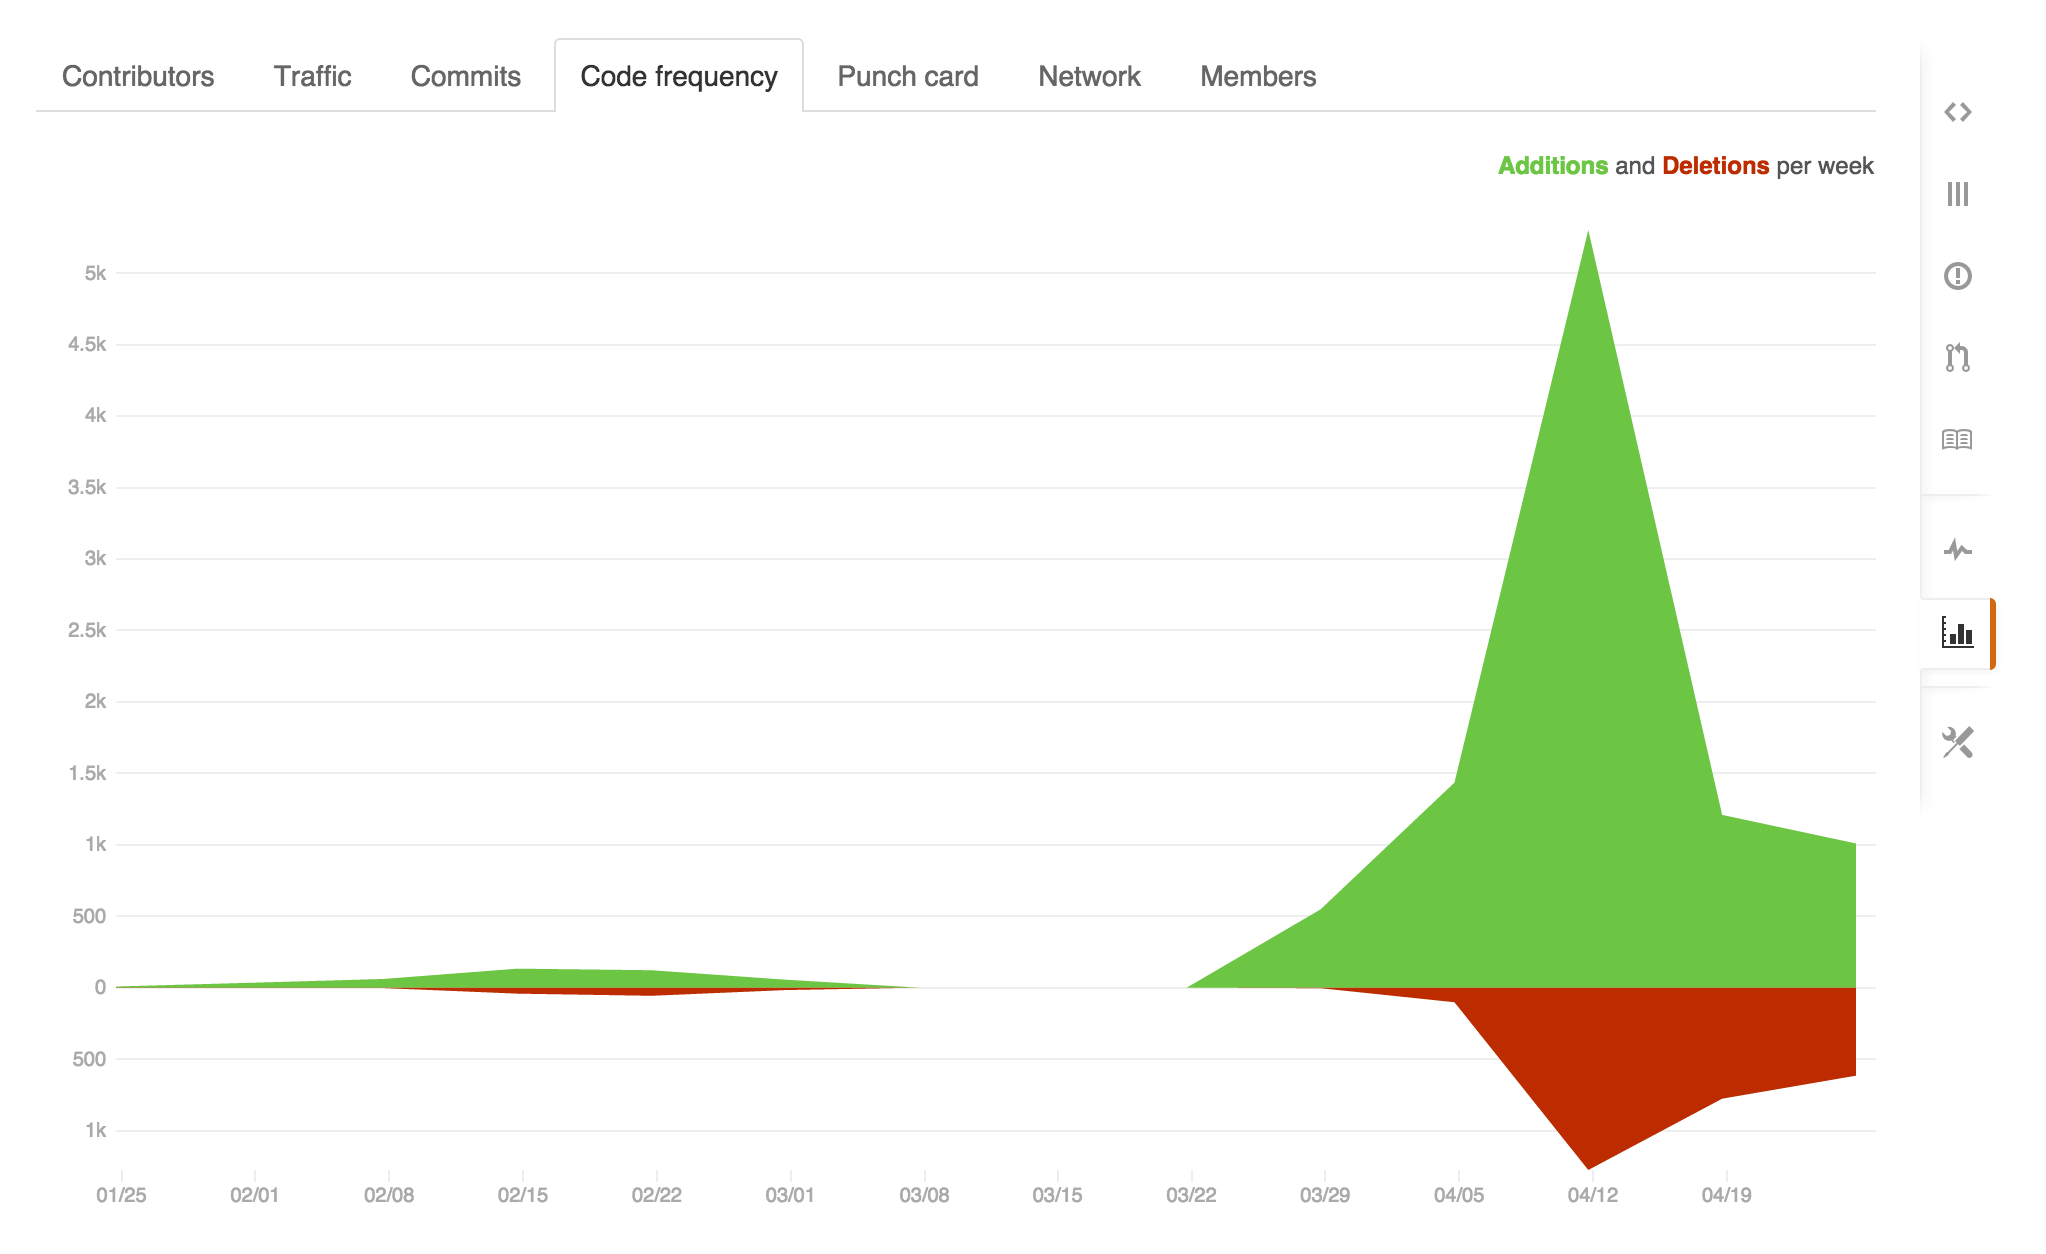
\includegraphics[width=4.5in]{codefrequency.png}
        \caption{Github Code Frequency.}\label{code:freq}
\end{figure}

\begin{figure}[H]
        \centering
        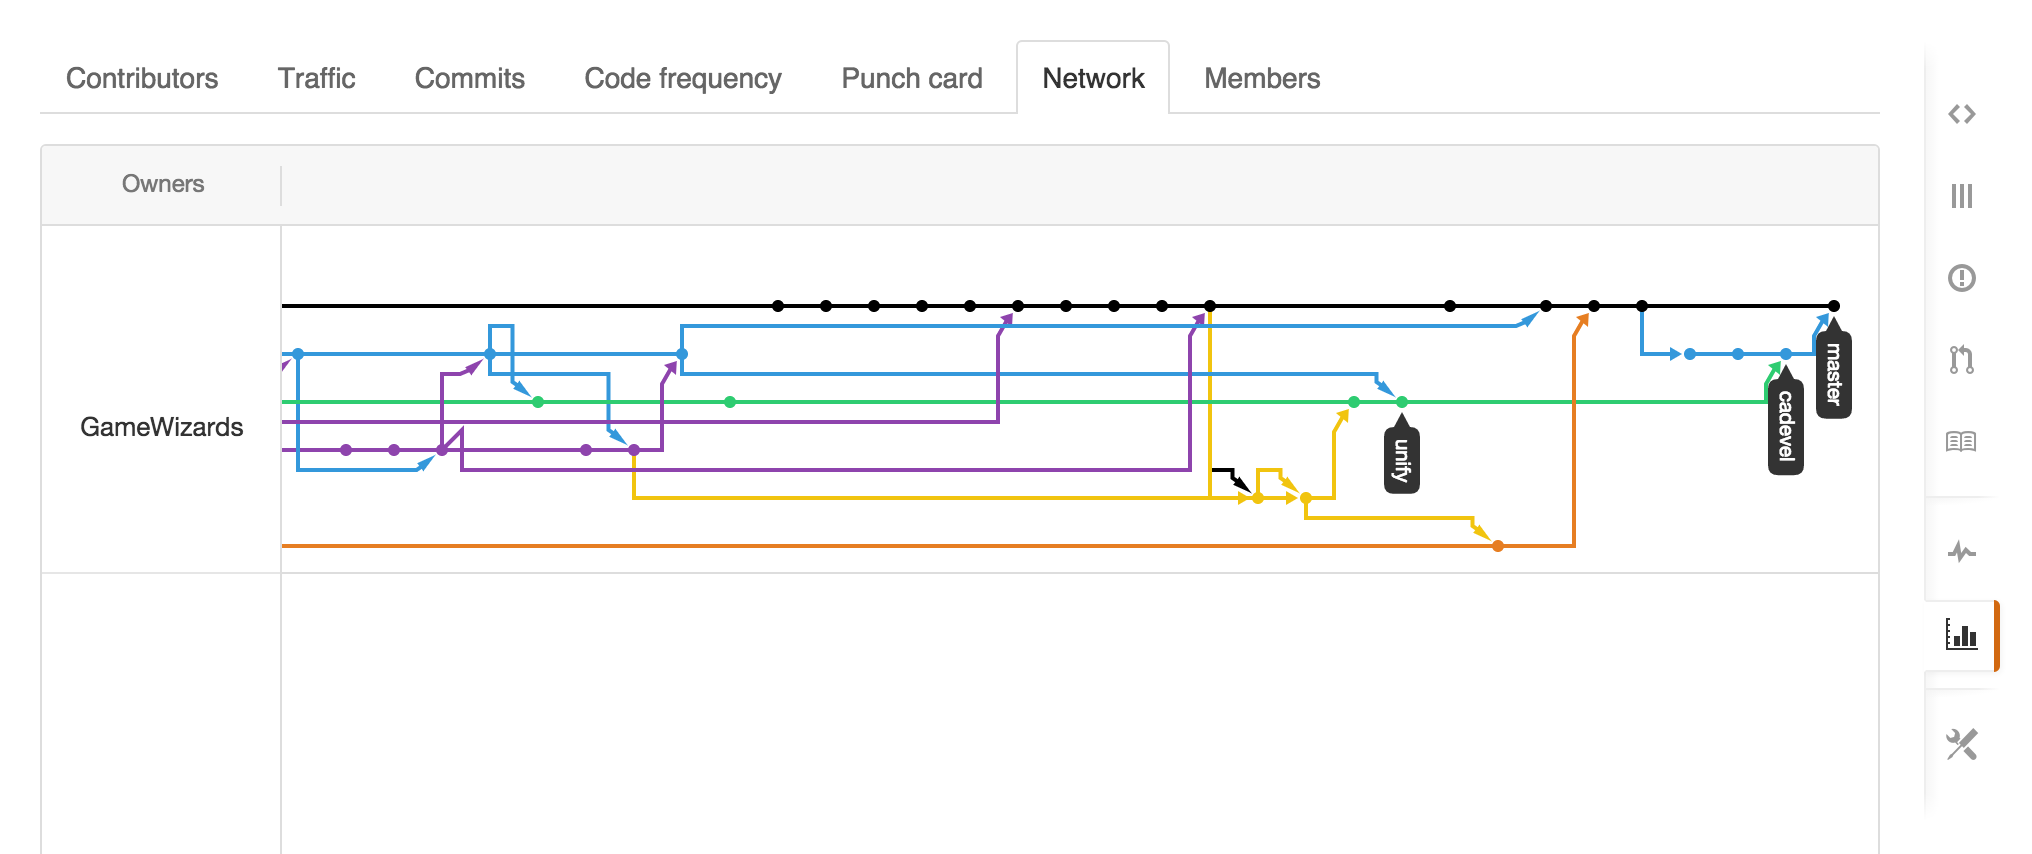
\includegraphics[width=4.5in]{networkgraph.png}
        \caption{Github Network Graph Tail.}\label{code:graph}
\end{figure}

\begin{figure}[H]
        \centering
        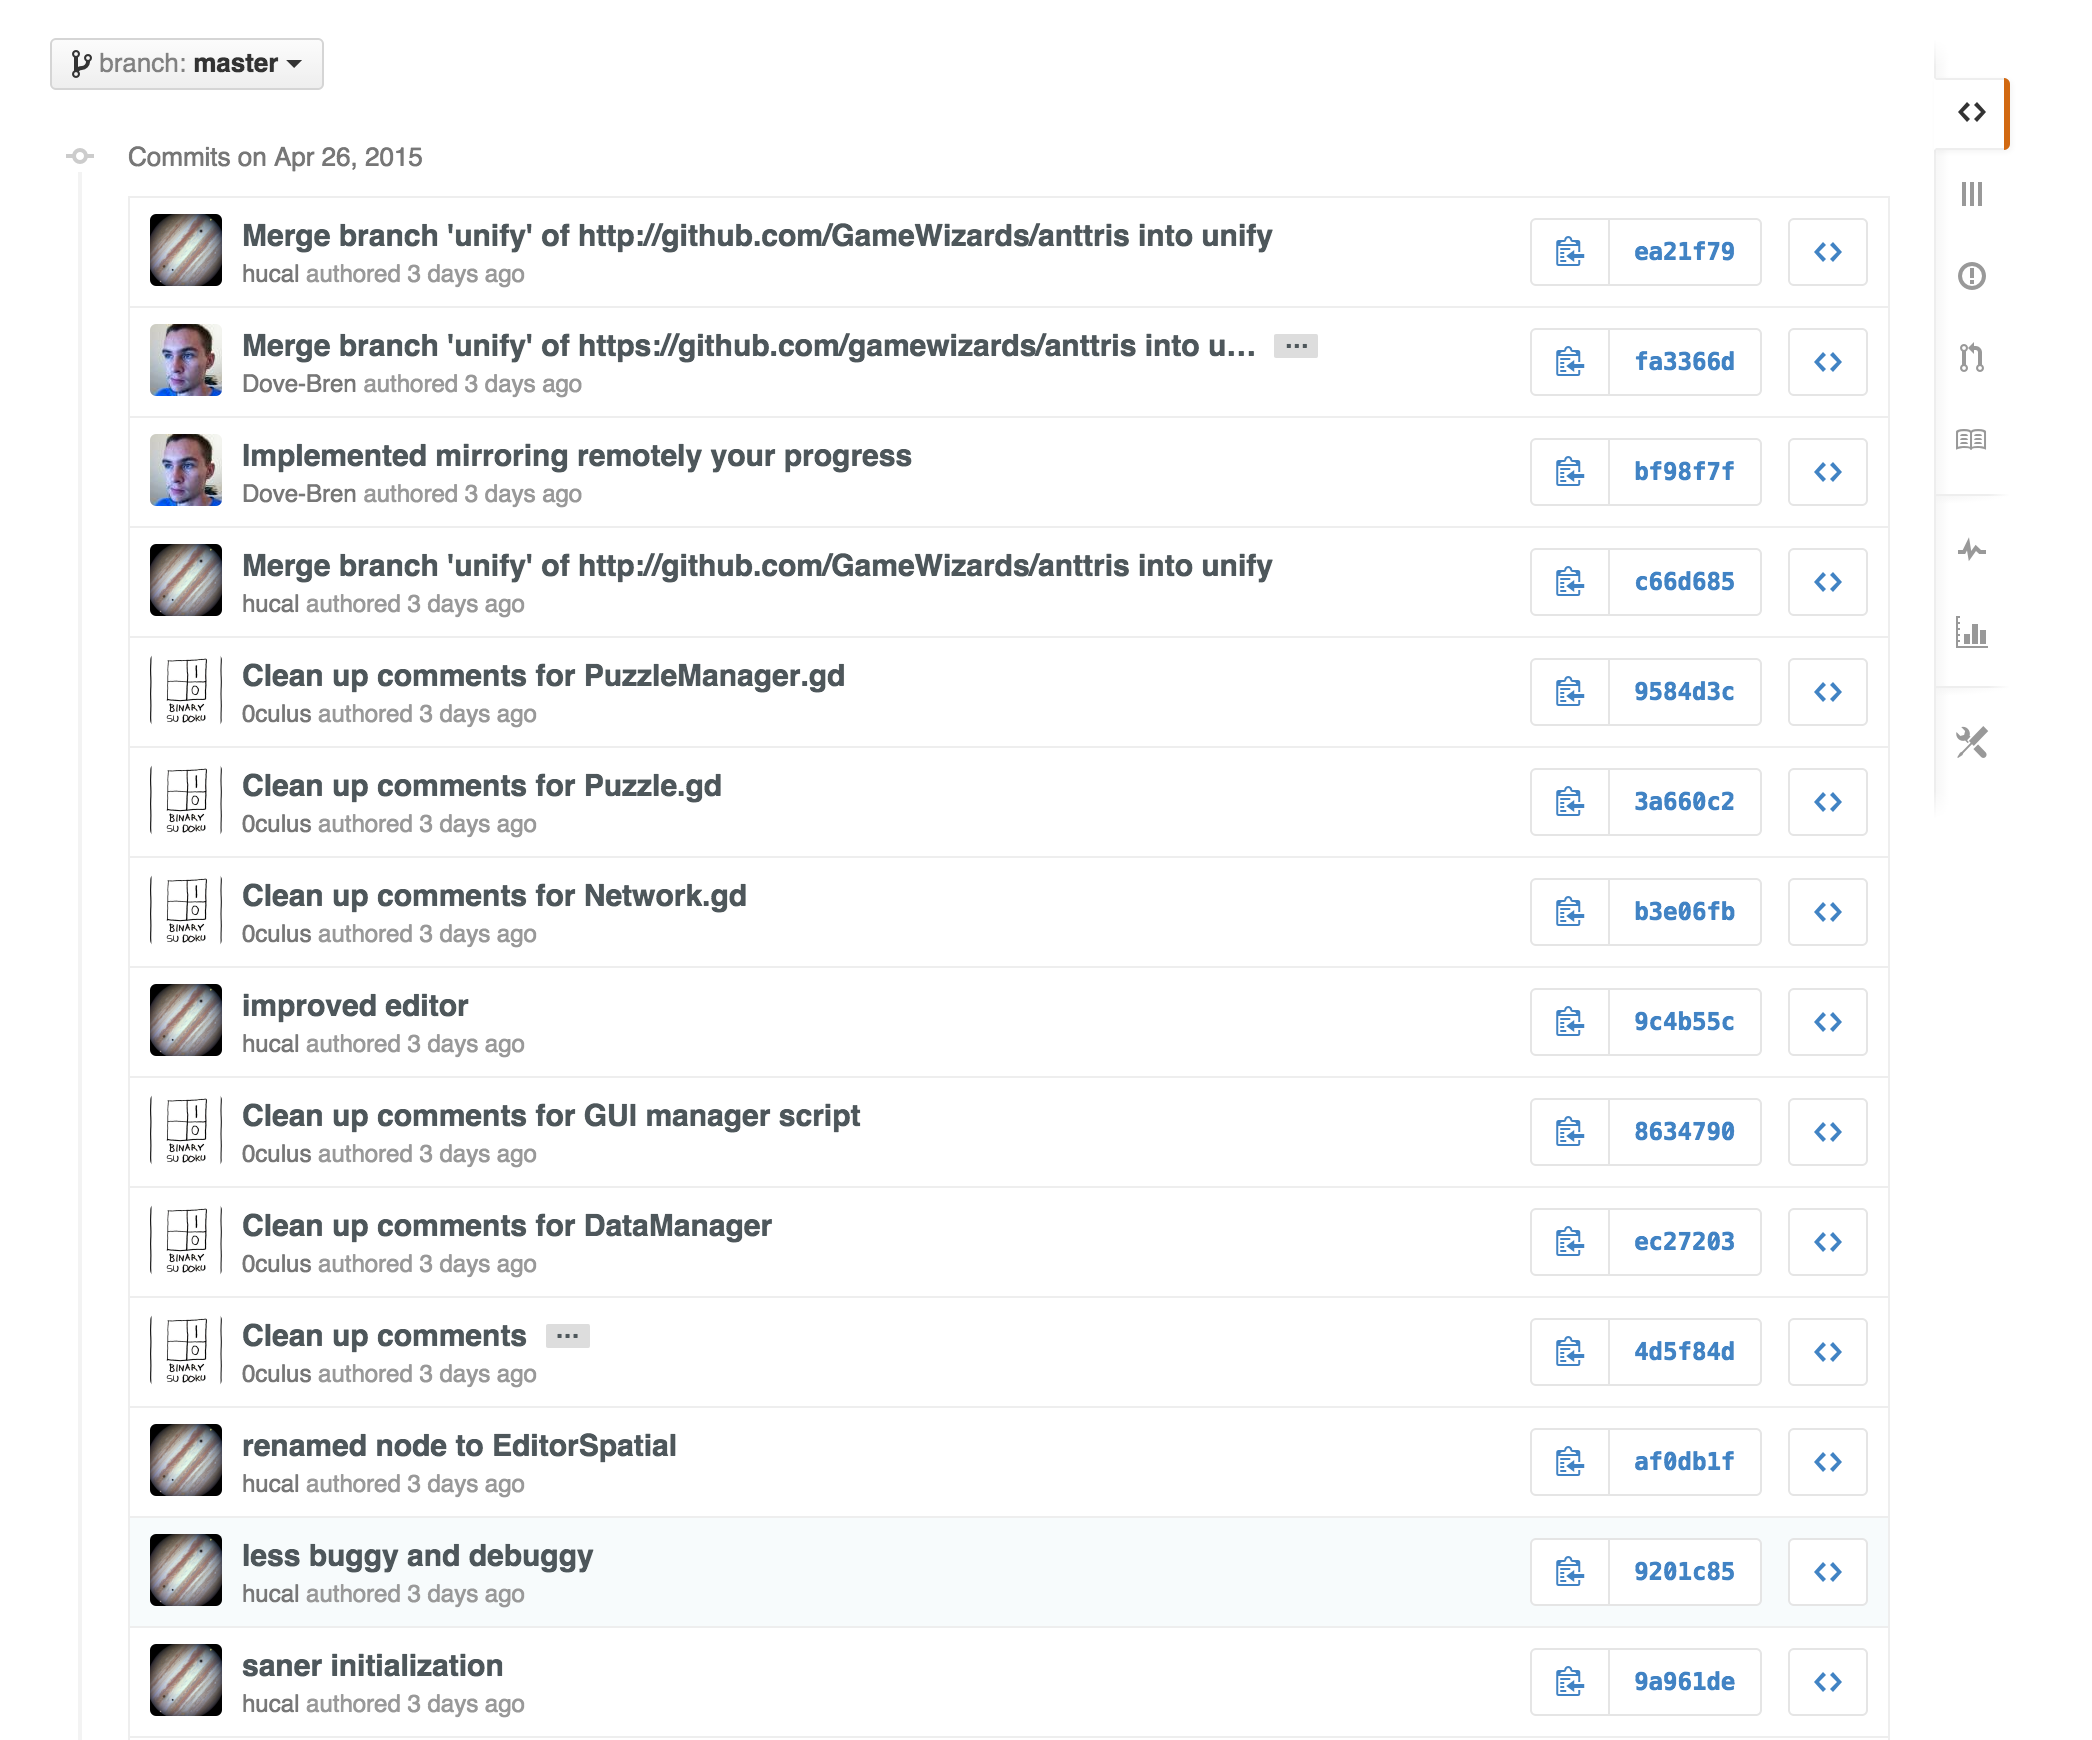
\includegraphics[width=4.5in]{commitsexample.png}
        \caption{An Example of Commits to master.}\label{code:commits}
\end{figure}

\begin{figure}[H]
        \centering
        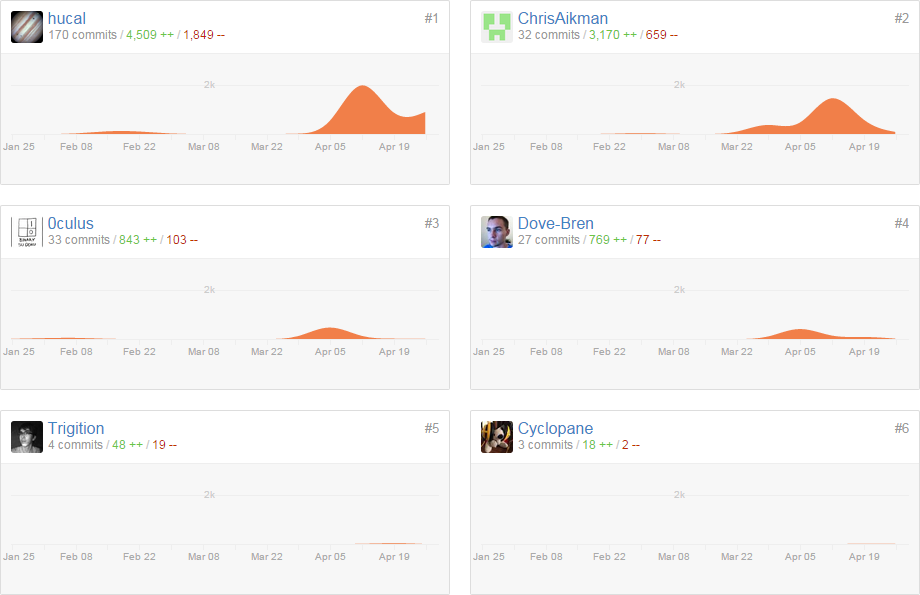
\includegraphics[width=4.5in]{CommitStats.png}
        \caption{Total commits sorted by additions.}\label{code:commitstats}
\end{figure}

As for Slack statistics, we are approaching 10,000 messages sent in total. We have multiple integrations, including Travis CI, Github, and Google Docs, as shown in Figure \ref{slack:stats}. Figure \ref{slack:window} shows an example of our Slack chat.

\begin{figure}[H]
        \centering
        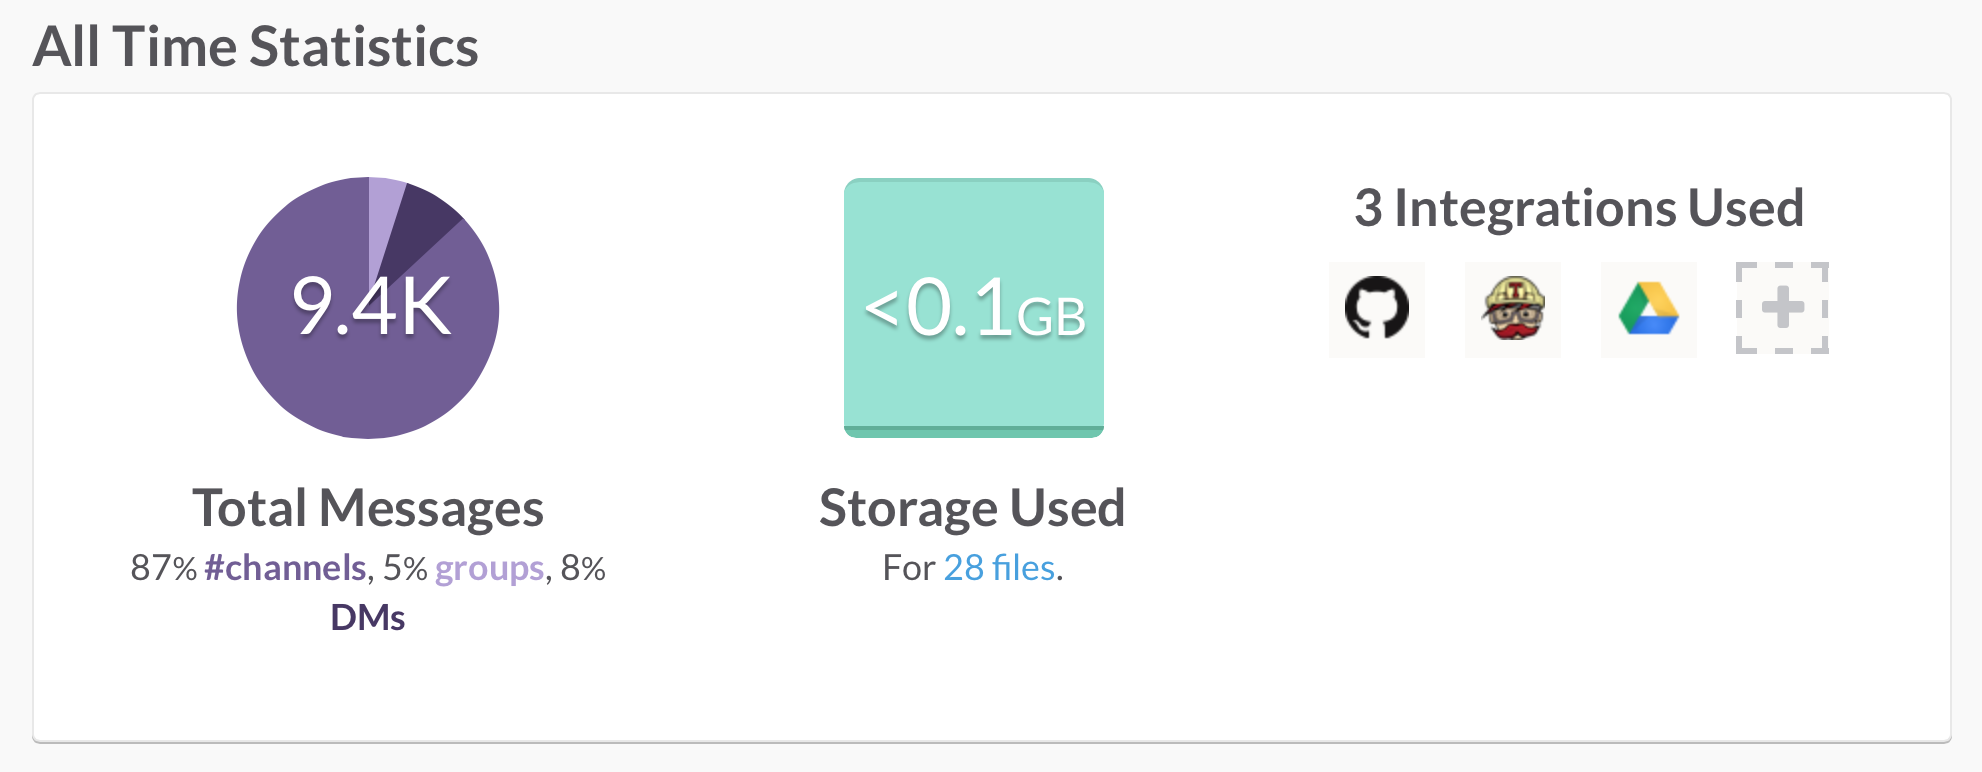
\includegraphics[width=4.5in]{slack.png}
        \caption{Our Global Statistics as Reported by Slack.}\label{slack:stats}
\end{figure}

\begin{figure}[H]
        \centering
        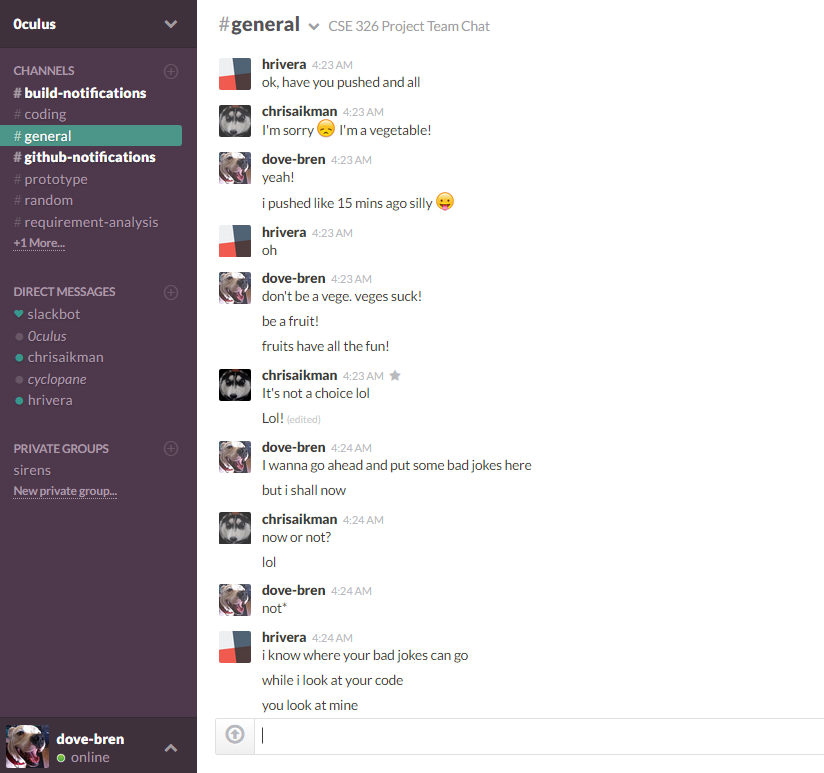
\includegraphics[width=4.5in]{slack-window.png}
        \caption{Our Slack.}\label{slack:window}
\end{figure}


\subsection{Project Schedule} % BENJI
%(I.e., an updated Gantt Chart)
\section{Appendices}
% Source code, java-doc version of your classes, etc






\bibliographystyle{acm}
\bibliography{team5-final-report}
\end{document}
